

\newcommand\dive{\textmd{div}}
\newcommand\der{\textmd{d}}




\chapter{Introduction}
%some background on all astronomy/astrophysics

Humans have been captivated by the stars since the dawn of civilisation, and this fascination has driven our curiosity and drive to understand the universe around us. 
The history of astronomy is rich and diverse. 
Indigenous cultures still use the stars for navigation, seasonal calendars, and mythological stories. 
Since the invention of the modern telescope, some would say the birth of modern astronomy in the 16th century, to the launch of the James Webb space telescope, technology has advanced during the period that this PhD was undertaken. 
Our ability to observe and study the stars has grown in scale and sophistication. 

Each observation that we make improves our understanding of the underlying physics of the universe. 
In recent years the sheer amount of data available to astronomers has increased dramatically due in part to technological advances, such as space-based observatories, which allow us to perform large sky surveys in unprecedented detail. 
It is clear from these studies that our models of the universe are lacking in a number of important physical processes. 
One of these physical processes that are particularly not well understood is the evolution of stellar rotation\footnote{Infact a majority of models of stellar evolution completely ignore angular momentum transport}.

This introductory chapter is intended to provide context for the reader to understand the following science chapters. 
The introductory chapter is broken down into the following sections of increasing level of detail:

Section \ref{sec:history} provides a historical overview of the history of astronomical observation and briefly introduces the techniques used to observe the rotation of stars.
Section \ref{sec:evolution} reviews our current understanding of the evolution of rotation from birth, through post-main-sequence evolution, to the remnants of rotating stars. Within this Section we also describe what we call the "problems of stellar rotation" that we have attempted to address in this work.
Section \ref{sec:effects} describes the astrophysical effects of rotation on stellar evolution.
% Section \ref{sec:techniques}  outlines the techniques that are employed to observe the rotation of stars.

The scientific works in this thesis are motivated by the problems in stellar rotation that are described in detail in this introduction. As a result, this introduction will overlap with the introductions of the scientific works' topics and serve as a companion for readers unfamiliar with the topic.

\section{History of observation of rotation}
\label{sec:history}

In this section, we look back at the history of observing stellar rotation, how observations of stellar rotation are performed, the qualitative effects of rotation on stellar rotation and some of the problems that the big-data boom of astronomy has identified.
This discussion will provide the necessary background to our attempts to understand and constrain the astrophysical process that underlies these problems.

The history of observing the rotating stars began with observations of the Sun\footnote{as most astronomy does}. 
In approximately 1610, Galileo reported evidence of sunspots and tracked their motion in his book "l'Istoria e dimostrazioni intorno alle macchie solari e loro accidenti". 
He interpreted the motion of stellar spots on the surface of the Sun as a result of its rotation. 
Adding onto this work in 1630, Christoph Scheiner found that the stellar spots had different rotational periods at the poles and the equator - measurements that agree with modern observations of the Sun. 
This was the first observation of latitude-dependent rotation - more commonly known as latitudinal differential rotation. 

The history of observing stellar\footnote{Here we make the distinction between the Sun and other stars through the use of the terms' solar' and 'stellar' respectively} rotation can be traced back to the early 20th century when astronomers first discovered that some stars they observed were rotating. 
They came to this conclusion through spectroscopic observations \citep{elvey_contours_1929, struve_stellar_1930, struve_axial_1930}.
They found that lines in their spectra were broadened due to the Doppler effect - a technique used to this day.


Around this time, astrophysicists such as Eddington \citep{eddington_conditions_1918,eddington_internal_1926,eddington_internal_1929}, Milne \citep{milne_equilibrium_1923}, von Zeipel \citep{von_zeipel_radiative_1924}, and others delved into the theoretical aspects of the impact of rotation on stars.
To simplify their work, they identified the effects of rotation on stellar structure, energy generation, shape and luminosity. 
Further, rotation induces mixing in stars that can transport angular momentum as well as elements.
Advances in computational capabilities allowed astronomers to study the impact of rotation on the mixing of elements within stars in greater detail. 
This research revealed essential results: rotation significantly impacts the mixing of matter in stars. 
Enhanced mixing leads to an increased lifetime on the main sequence - hydrogen-rich material is transported to the core - and can create isotope anomalies, such as changes in the isotopic ratio $^{12}$C/$^{13}$C, nitrogen, oxygen and lithium enhancements \citep{maeder_evolution_2000,heger_presupernova_2000,charbonnel_lithium_1994}.
Their results underlay our modern understanding of the impacts of stellar rotation on stellar evolution.

In the following decades, technological advances allowed for more precise photometric observations of stars. This paved the way for two techniques to obtain measures of the rotation of stars - stellar spot brightness modulation periods and asteroseismology.

Like with the Sun, stars were found to exhibit stellar spots. These spots cannot be realistically tracked on the surface of stars other than the Sun. 
They do, however, vary the star's observed brightness.
With stellar spots tied to the star's rotation, these brightness variations are periodic. 
Measuring the period of brightness variation is used as a proxy for the rotation period\footnote{It is important to note here that the rotation period - time taken for one rotation -  and rotation rate - frequency of rotation - of a star are not the same quantity. They are inversely related} of a star. Unlike the spectroscopic technique - where the inclination angle modulates the rotation rate  - the rotational periods from stellar spot brightness modulations are more accurate to the star's actual rotation rate.
As a result, this technique has made several fundamental discoveries about the evolution of stellar rotation.
The accurate measurement of stellar rotation provides information to more accurately model a star's internal structure, dynamics and internal angular momentum transport - both at a specific point in evolution and with evolution.
For example, it was found that the rate at which a star's surface rotates slows with time \citep{skumanich_time_1972}.
Resultingly, measuring the stellar rotation can provide an imprecise measure of the age of a star \footnote{This is a contentious claim that we will discuss further in the coming sections}. Recent photometric missions such as \kepler{} \citep{borucki_kepler_2010,beck_kepler_2011}, Zwicky Transient Facility (\ZTF) \citep{lu_bridging_2022} and \gaia{} \citep{distefano_gaia_2022} have provided a wealth of data, including a sample of ~200,000 stellar rotational periods from stellar spot brightness modulations. Their results form the basis of a number of the problems in stellar rotation we discuss in this thesis. 

Determining the rotation period of a star from stellar spots requires intermittent photometric measurements of stars - known as long-cadence observations - over the time scale of months. 
On the other hand, measurements made on the order of minutes - known as short cadence observations - reveal the internal structure of stars.
Like bells, stars "ring" - or, more accurately, pulsate and thus vary in brightness -  at particular frequencies related to the structure of the star.
By measuring those frequencies, we can infer the internal structure of a star - for example, the density-sound speed profile of the star.
Rotation introduces what are known as rotational splittings to the frequency profile.
Rotational splittings vary between asteroseismic modes but are a weighted average of the rotation rate dependent on the structure of the star. 
Unlike brightness modulations from stellar spots and spectroscopic inference of rotation rate, asteroseismology can probe the rotation profile internal to the surface of a star.

Modern observations with asteroseismology\footnote{and helioseismology for the Sun} have also found that the Sun, and most post-main-sequence stars, exhibit differential rotation along the radial axis - known as radial differential rotation.
Measurement of the rotation profile of post-main-sequence stars has allowed us to probe these stars' internal mixing and angular momentum transport. 
It is important to note, however, due to the large amount of photometric data required to perform in-depth asteroseismic inference, the number of stars it has been performed on is only on the order of 100\footnote{at the time of writing} \citep{li_asteroseismology_2020,li_asteroseismology_2020-1}, and the constraints that state-of-the-art data can provide are limited. We would argue that the information that asteroseismology has provided has introduced more questions than currently answered.

The study of stellar rotation continues to advance and remains at the forefront of current research.

\section{Evolution of rotation}
\label{sec:evolution}

\subsection{Birth - Terminal age main sequence}

Before we discuss the observed evolution of rotation along the main sequence, we will briefly reflect on the methods of observing rotation in stars, where these methods are most conducive to understanding the evolution of rotation and their limitations.
The three standard techniques of observing rotation in stars can be separated into three categories: measurement of the surface rotation period from stellar brightness oscillations owing to stellar spots, spectroscopic derivation of inclination projected surface velocity from doppler broadenings, and asteroseismology of rotational splittings.
We will refer to these techniques by their data products: stellar spot rotation periods, spectroscopic rotation velocities, and asteroseismic rotation rates, respectively, for brevity.
% We discuss these techniques more thoroughly in Section \ref{sec:techniques}.
The results we discuss in this Section come from the inference of rotational evolution from stellar spot rotation.
This results from two factors: stellar spot rotation periods are more accurate and less data andcomputationally intensive than their spectroscopic and asteroseismic counterparts.

While the spectroscopic rotation velocity has been inferred for orders of magnitude greater numbers of stars, the observed rotation rate is modulated by the inclination angle of the star relative to the observer ($v\sin{i}$).
Constraining the evolution of rotation through spectroscopic rotation velocities of stars is only fruitful with independent constraints to stellar inclination.
The stellar inclination is often difficult to measure as it requires either that the star is in a binary\footnote{and that the rotation axis aligns itself with the binary orbital inclination, which may always be the case \cite{albrecht_banana_2011,albrecht_banana_2013}} or that the star is intensively asteroseismically studied.
As a result, only a few studies of the evolution of rotation rely on this data.

% Interestingly stellar spot rotation periods and spectroscopic rotation velocities seem to disagree.
% This is shown in Figure \ref{fig:rot_periods_spectroscopic_disagree}.
% While it is expected that the spectroscopic surface rotation periods should be larger than their stellar spot rotation periods, as a result of the inclination projection,.

%TODO MAKE THE PLOT AND CHECK BEFORE WRITING

On the other hand, determining the rotation rate of stars with asteroseismology is computationally and data-intensive.
We will discuss the difference in computational intensity in more detail when we outline how these methods are performed.
Here we will focus on the difference data intensity.
Obtaining high signal-to-noise asteroseimic signals of rotation requires short-cadence observations of stars over an observation period of ~4 years \citep{deheuvels_seismic_2014}. 
Short-cadence data is required because the oscillation frequencies of main-sequence stars must be greater than the Nyquist frequency of the observations.
In the \kepler{} field, the cross-section of stars with both short-cadence observations and those observation periods long enough to obtain a high enough SNR to perform asteroseismic inference is very limited.
Further, only limited constraints can be placed on the surface rotation rate from asteroseismology during the main sequence.
Main-sequence stars only express p-mode\footnote{See Section \ref{sec:asteroseismology}} solar-like oscillations with long lifetimes, which can only probe the structure of the convective surface region.
Long mode lifetimes result in wide line widths of oscillations in the power spectrum.
Main-sequence stars spend the majority of their lifetime slowly rotating.
This results in rotational broadenings of the oscillations rather than distinct rotational splittings.
Without precise measurements of the rotational splittings for many oscillation modes, precise inference of the surface rotation rates of main-sequence stars is limited.

The inefficiency of asteroseismic inference of rotation rates along the main sequence is best exhibited in \citet{hall_weakened_2021}, who observed the asteroseismic surface rotation rates of 91 main-sequence stars.
Figure 2. in \citet{hall_weakened_2021}compares the stellar spot rotation period with the surface rotation period from asteroseismic inference of the rotation profile.
The surface rotation periods generally agree, confirming that the surface brightness oscillation period from stellar spots is indeed the surface rotation period.
However, the rotation periods obtained from asteroseismology are much less precise than their stellar spot rotation period counterparts.
Despite requiring much more data, the information provided by this technique is limited compared to stellar spot brightness modulation periods.

Stellar spot rotation period measurements can be made from long-cadence data with observation periods as low as 90 days \citep{mcquillan_rotation_2014}.
The technique employed to determine the rotation period is much less computationally intensive than required for asteroseismic inference of rotation rates.
As a result and through the combination of various photometric missions, \kepler{} \citep{mcquillan_rotation_2014, santos_surface_2021}, \ktoo{} \citep{santos_surface_2021}, Zwicky Transient Facility (\ZTF) \citep{lu_bridging_2022}, \gaia{} DR3 \citep{distefano_gaia_2022} %todo reference% ~500,000 stars have had their stellar spot rotation periods measured.
We show the rotational period distribution against colour (Gaia DR3 $B_P - R_P$) of the \kepler{} Mcquillan Sample, \ZTF{} sample and \gaia{} DR3 samples in the top, middle and bottom panels of Figure \ref{fig:rot_comp} respectively.

\begin{figure}[h]
    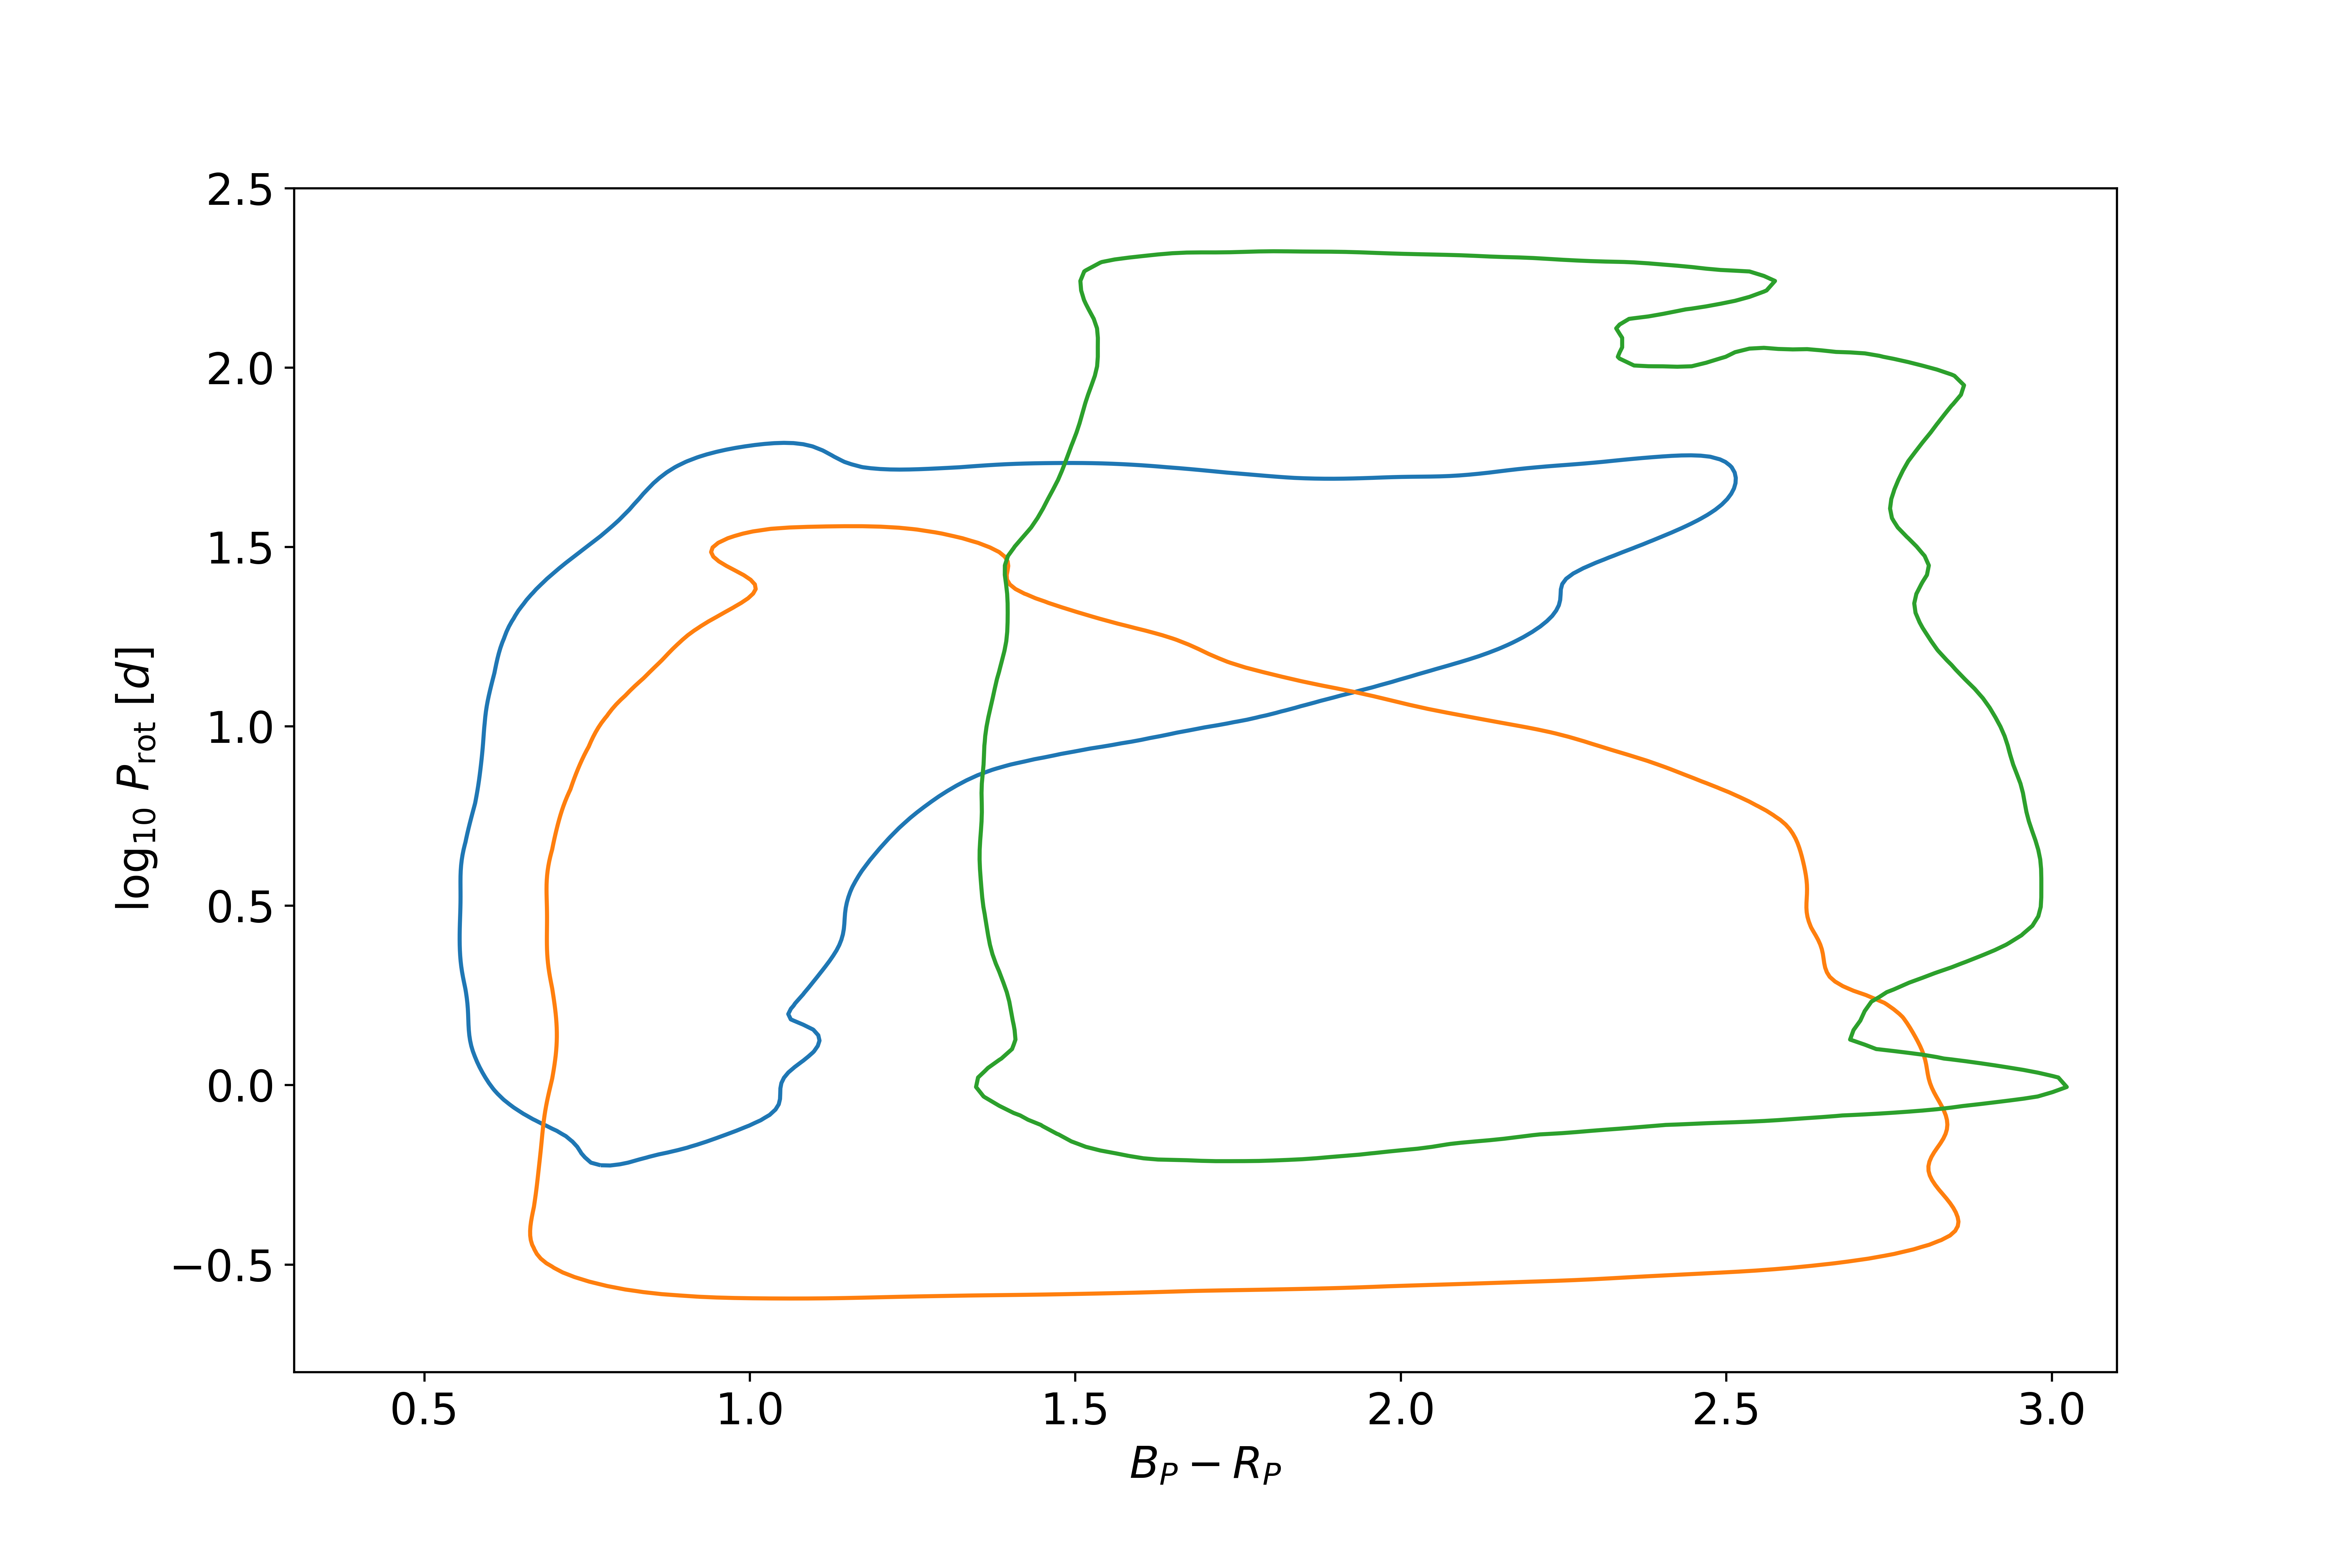
\includegraphics[width=\textwidth]{Figures/intro_figures/rot_comp.png}
    \caption{Normalised 2D histograms of the \kepler{} \citep{mcquillan_rotation_2014} (Top), \gaia{} DR3 \citep{distefano_gaia_2022} (Middle), and Zwicky Transient Facility (\ZTF) \citep{lu_bridging_2022} (Bottom) samples. Each sample probes a different area of the rotational period against colour space with some overlap. This expands our knowledge of the evolution of rotation to different types of stars while the agreement between these samples confirms their independent accuracy.}
    \label{fig:rot_comp}
\end{figure}

The stellar spot rotation periods that are obtained from each of these missions are suited to observe particular masses and rotation period regimes along the main sequence.
This results from the underlying telescope parameters, the scanning technique employed, and each mission's observation cadences \citep{distefano_determination_2012}.
Comparing the rotational period distributions in Figure \ref{fig:rot_comp} we observe a few notable features and limitations from each mission.
The Gaia DR3 rotation period sample exhibits spurious periods centred around 0.5, 18, 25, 32 and 49d.
\citet{distefano_gaia_2022} suggest that the non-uniformity of the Gaia sampling could be the cause of these peaks.
\kepler{} mainly targeted solar-like stars.
As a result, in the \kepler{} sample, there is a lack of measured periods for M dwarfs and fast-rotating young stars.
On the other hand, the \ZTF{} and \gaia{} samples did not have this targeting bias.
As a result, the \ZTF{} and \gaia{} samples probe the rotation periods of the comparatively lower-mass (redder) stars.
The Gaia DR3 rotation sample is, as a result of the Gaia scanning law, mostly suited to detect periods of rapidly rotating stars (P $<$ 5 d).
Due to the long observation baseline, the \ZTF{} mission was more suited to observe longer rotation periods.
Combining the results of these missions, we can accurately probe the evolution of rotation along the main sequence for a wider range of stellar parameters than the individual missions permit.
Further, the cross-match of stars between these missions confirm whether the individual missions themself provide accurate measures of the stellar surface rotation period.

Most of what we know about main-sequence rotational evolution arises from measuring stellar spot rotation periods.
However, the technique is limited by the requirement for stars to express stellar spots to be effective - a limitation that is invoked several times to explain phenomena discussed later in this Section. 
\citet{mcquillan_rotation_2014} attempted to measure the stellar spot rotation periods of solar-like stars in the \kepler{} sample.
In this work, they recovered the rotation period of ~20\% of stars with long cadence observations -~34000 detected rotation periods out of ~133000 selected stars in the sample.
On the other hand, \citet{distefano_gaia_2022} places the efficiency of the Gaia DR3 period detection pipeline at ~0.4\%.
They argue that the detection efficiency is non-constant and, in fact, a function of stellar magnitude, the amplitude of the rotational modulation, the stellar rotation period and the ecliptic latitude.
There may be regions of evolution where the stellar spot rotation period does not effectively probe rotational evolution.

All matter in the universe has some angular momentum. 
Stars are born in the core of spinning molecular clouds from the infall of matter due to gravity. 
As a result, all stars are rotating.
The amount of angular momentum a star is born with may depend on the cloud from which it was formed.

At the beginning of the  pre-main-sequence (PMS) phase, a young star is typically surrounded by a disk of gas and dust from which it is accreting material.
The accretion process can lead to an increase in the rotation rate of the star, as the angular momentum of the infalling material is transferred to the star.
However, as the star grows in size and mass, its magnetic field becomes stronger, which can slow down its rotation through the process of magnetic braking.

One key feature of PMS rotational evolution is the "disk-locking" phenomenon, in which the star's rotation becomes locked to the rotation of the disk \citep{eggenberger_angular_2012}.
This occurs when the star's magnetic field is strong enough to interact with the disk, causing the star and disk to rotate together.
Disk-locking can help to explain why some PMS stars have relatively long rotation periods, even though they are young and should be rotating rapidly due to the effects of accretion.

The interplay between accretion and magnetic braking can result in a complex evolution of the rotation rate of a young star during the PMS phase \citep{gallet_improved_2013}.
Observations of young stars in star-forming regions have revealed that the rotation rates of PMS stars span a wide range, with some stars spinning rapidly and others rotating slowly.
We show this complex relationship in Figure \ref{fig:pms_ms_evo}.
Comparative to the main-sequence where stars generally spin-down due to surface winds, the median rotation rate of PMS cluster is relatively constant with age.

\begin{figure}
    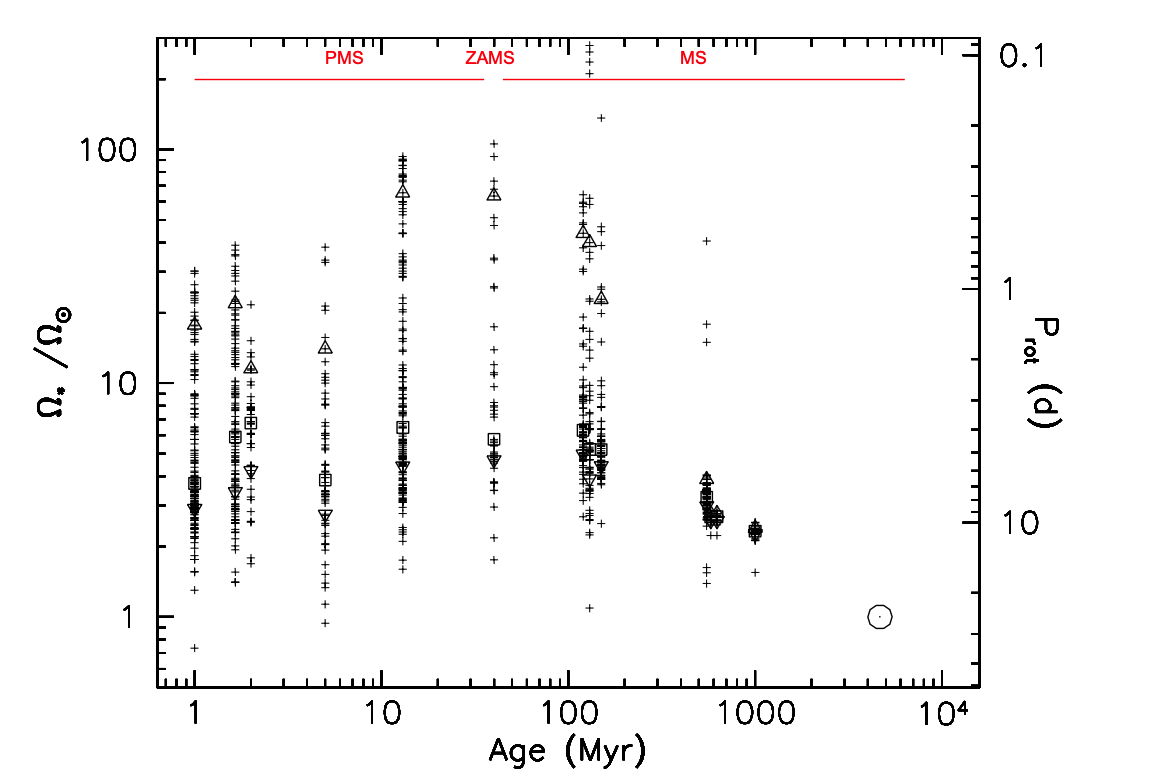
\includegraphics[width=\textwidth]{Figures/intro_figures/pms_evo.png}
    \caption{Angular rotation rate (relative to solar) distributions of low-mass young open clusters and the Sun. Triangles, inverted triangles, and squares represent the $90^{th}, 25^{th},$ and median rotation rates of the cluster. Open circle denotes the present value of the rotation rate of the Sun. Median values indicate that the rotation rate of cluster is approximately constant with age, despite the spin up by accretion. In order of increasing age (left to right) the clusters are ONC (1 Myr) \citep{herbst_stellar_2002}, NGC 6530 \citep{henderson_time-series_2012}, NGC 2264 (2 Myr) \citep{affer_rotation_2013}, NGC 2362 (5 Myr) \citep{irwin_monitor_2008}, h PER (13 Myr) \citep{moraux_monitor_2013}, NGC 2547 (40 Myr) \citep{irwin_monitor_2008}, Pleiades (120 Myr) \citep{hartman_large_2010}, M50 (130 Myr) \citep{irwin_monitor_2009}, M35 (150 Myr) \citep{meibom_slar_2009}, M37 (550 Myr) \citep{hartman_deep_2009}, Praesepe (578 Myr) \citep{delorme_stellar_2011}, Hyades (625 Myr) \citep{delorme_stellar_2011}, and NGC 6811 (1 Gyr) \citep{meibom_kepler_2011}.  Sourced from \citet{gallet_improved_2013},  Figure 1.}
    \label{fig:pms_ms_evo}
\end{figure}

While the many main-sequence stars have had their rotation rates measured, their ages are not well-constrained.
Resultingly the evolution of rotation with age is also not well-constrained.
Observations of young open clusters' main-sequence surface rotation from the \kepler{} mission suggest that angular momentum transport over a star's lifetime is consistent between clusters - the distribution of rotational periods of stars has considerable overlap between clusters \citep{spina_how_2020, curtis_when_2020}. 
Figure \ref{fig:cluster_rotational_periods} shows the distribution of rotation rates of some open clusters.
In this Figure, we can observe some significant aspects of the evolution of angular momentum in stars.

\begin{figure}[h]
    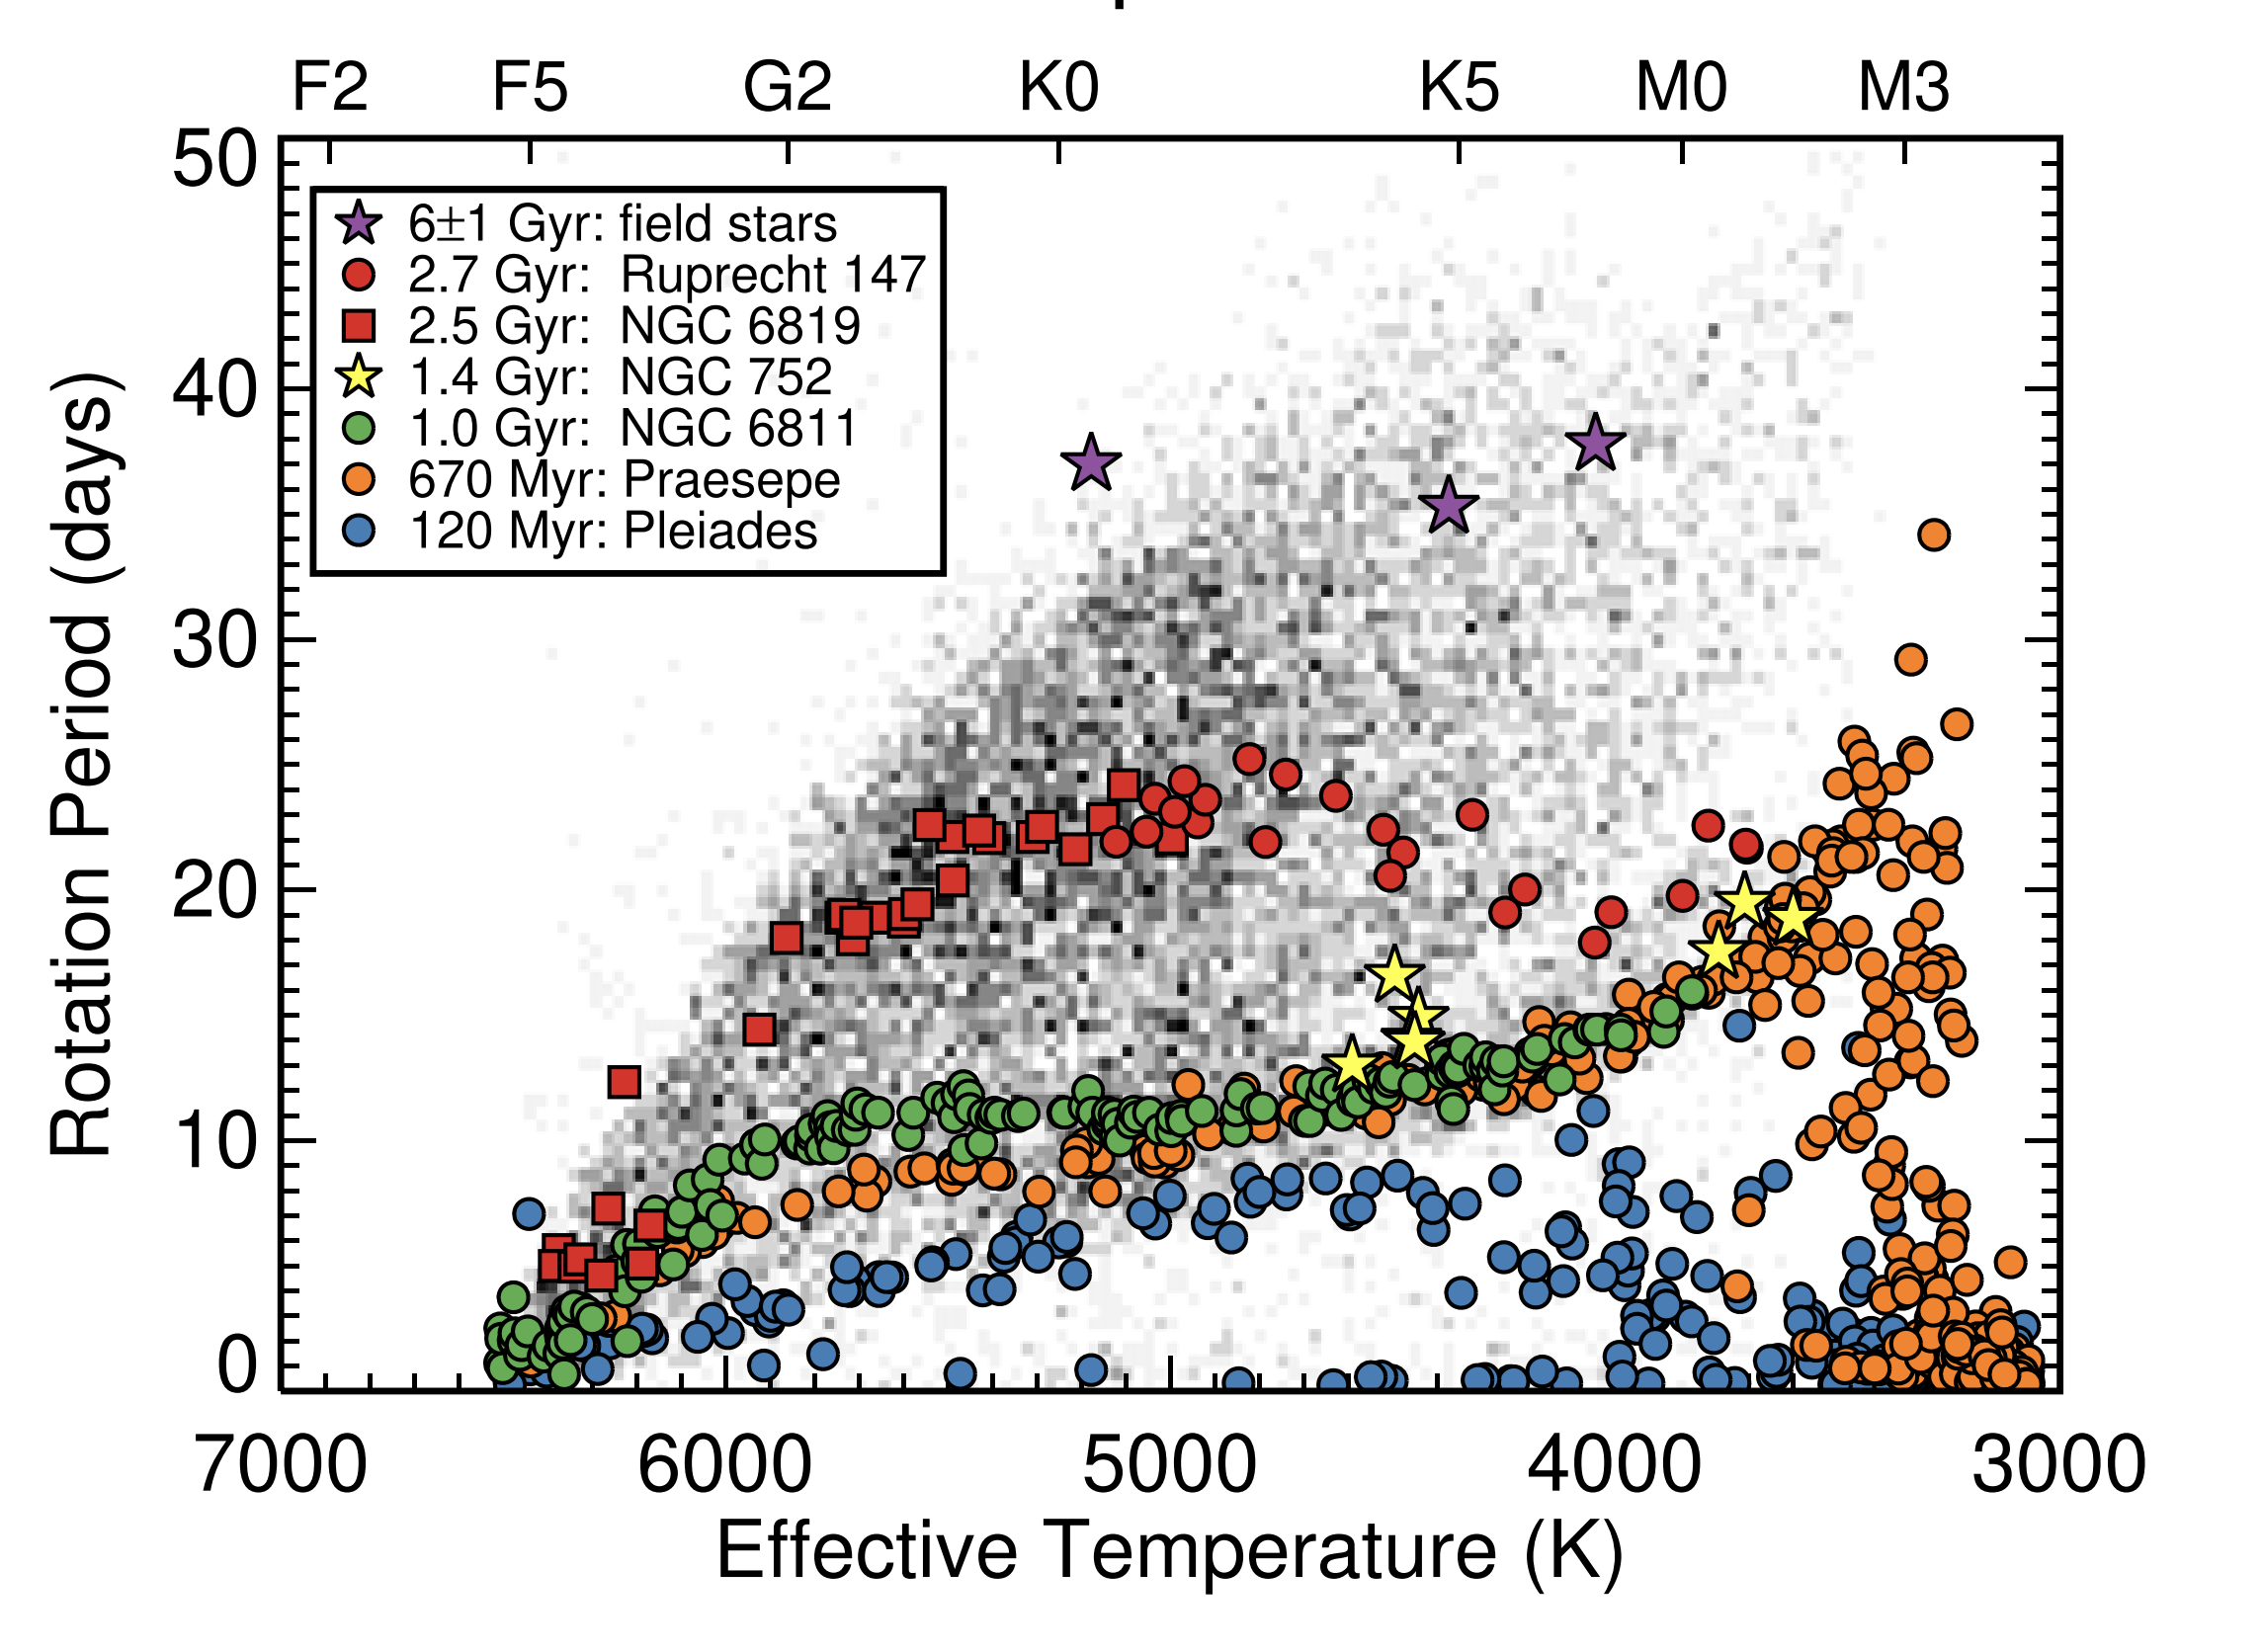
\includegraphics[width=\textwidth]{Figures/intro_figures/cluster_kepler.png}
    \caption{Scatter plot of various cluster rotational periods against effective temperature overlayed on the \kepler{} \citet{mcquillan_rotation_2014} rotational period sample.
    The agreement between low mass Praesepe and NGC6811 periods implies mass dependent core-envelope coupling for young ($<$1 Gyr) stars.
    Sourced from Top left panel of Figure 7 in \citet{curtis_when_2020}}
    \label{fig:cluster_rotational_periods}
\end{figure}

The surface rotational period increases over time for stars between $<$1.1 $M_{\odot}$.
Within this range of masses, angular momentum is lost from the convective surface through mass loss and interactions of the star's magnetic field and the lost ionised material through stellar winds - magnetic braking.
Through observations of the Pleiades, Ursa Major, and Hyades stars and the Sun, \citet{skumanich_time_1972} derived the proportional relation between the rotational rate of stars and the inverse square of their age - $\omega(t) \propto t^{-1/2}$.
This proportionality forms the standard for expected rotational evolution and for what is known as gyrochronology - measuring the ages of stars from their rotational rate.

Outside the $\sim$0.4 and 1.1 M$_{\odot}$ range, the rotation period also decreases, albeit slower, with much more complex relationships with time.
Above $sim$ 1.1 M$_{\odot}$, known as the Kraft break, stars have shallower convective envelopes and are believed to have less efficient magnetic dynamos - which induce strong magnetic fields.  
Resultingly, the magnetic braking in these stars is less efficient, and these stars continue to rotate rapidly throughout most of their main-sequence lifetimes. 
Below 0.4 M$_{\odot}$ stars are fully convective.
Angular momentum is efficiently transported throughout the star.
A greater amount of angular momentum needs to be removed to slow the star's rotational rate, compared to stars that are not fully convective.
The main-sequence rotational evolution of stars with mass $>$1.3 M$_{\odot}$ is unprobed.
Above this mass, stars have no convective envelope, and thus, they do not express stellar spots nor solar-like oscillations that can be used to probe the surface rotation rate.
Theoretical modelling of the rotational evolution of high-mass stars is a substantial area of research in which observations of stellar parameters such as chemical abundances must independently constrain angular momentum transport rather than observations of stellar rotation.
As this work has a stronger focus on observing the rotation of stars, these results will not be discussed here.
For more information, we suggest reviews of astrophysical models of high-mass stellar rotational evolution, e.g. \citet{heger_presupernova_1998,maeder_evolution_2000,maeder_physics_2009}.

Until recently, it was assumed that there was little to no angular momentum transport between the radiative core and convective surface of main-sequence stars in the 0.4 - 1.1 M$_{\odot}$ range. 
Helioseismic observations of the Sun suggest that only the stellar surface undergoes rotational braking, and the core remains rotating rapidly - suggesting minimal angular momentum transport between the core and the surface on the main sequence. 
However, open cluster rotation period observations suggest that Skaumanich-like rotational evolution alone does not explain the observed distributions of rotation periods with mass.


\citet{spada_competing_2020} proposed that mass-dependent angular momentum transport between the core and the surface was required to explain observations of young ($<$ 1 Gyr) open cluster rotation period distributions.
In their work, they argue that clusters contain two sequences of stars: a sequence of relatively slower rotators, following the expected coherent slowing of rotation rate following the Skaumanich relation, and a sequence of lower mass stars that appear to have a constant rotation rate between clusters of different ages.
They compared the observations of the $\sim$700-Myr old Praesepe and the 1-Gyr old NGC 6811 clusters.
Figure 1 in \citet{spada_competing_2020} compares the rotation period distribution of the Pleiades (120 Myr), Praesepe (670 Myr), and NGC 6811 (1 Gyr).
Comparing observed rotation periods, they find that higher mass stars ($>$ 1 $M_{\odot}$) that are on the slow rotator sequence of the older NGC 6811 have longer periods than their counterparts in the younger Praesepe, as Skaumanich rotational evolution suggests.
On the other hand, the two clusters' rotational periods are indistinguishable at lower masses ($<$ 0.8 $M_{\odot}$)
In other words, low-mass stars have not been spinning down at all in the intervening 300 Myr. 
They argue that behaviour manifests mass-dependent core-envelope coupling - angular momentum transport between the core and the surface - briefly compensating for the loss of angular momentum due to wind braking at the surface.
They develop a semi-analytical model of the rotational period's evolution with a star's age and mass tuned with the observations of stellar cluster rotational period distributions.
This notably improves the accuracy of gyrochronology compared to the Skaumanich relation, especially for younger low-mass stars.

On the other hand the slow spin down rates of fast rotating stars could be related to saturation of the angular momentum loss due to stellar winds for fast rotating stars \citep{johnstone_stellar_2015, johnstone_stellar_2015-1,gallet_improved_2013}.
This is motivated by the saturation of magnetic field indicators for fast rotation rates - or rather low Rossby numbers \citep{wright_stellar-activity-rotation_2011}.
This could explain the slower observed spin-down of young rapidly rotating stars.
Both of these prescription neglect the each other: \citep{spada_competing_2020} includes a simple stellar wind prescription that does not consider the saturated regime, while \citep{gallet_improved_2013} does not consider mass dependent angular momentum transport within the star.

Another phenomenon not well explained by Skaumanich-like rotational evolution is the observed intermediate period gap.
\citet{mcquillan_rotation_2014} calculated the rotation periods of ~30000 stars in the \kepler{} sample from photometric oscillations of surface brightness from stellar spots.
The distribution of the log of the rotational periods from this sample against their colour is shown in Figure \ref{fig:kepler_rot_period}. 
Following increasing rotation period as a proxy for time, this Figure highlights the overabundance of observations followed, temporally, by a dearth of observations of particular rotational periods - the position of which varies with mass.

\begin{figure}[h]
    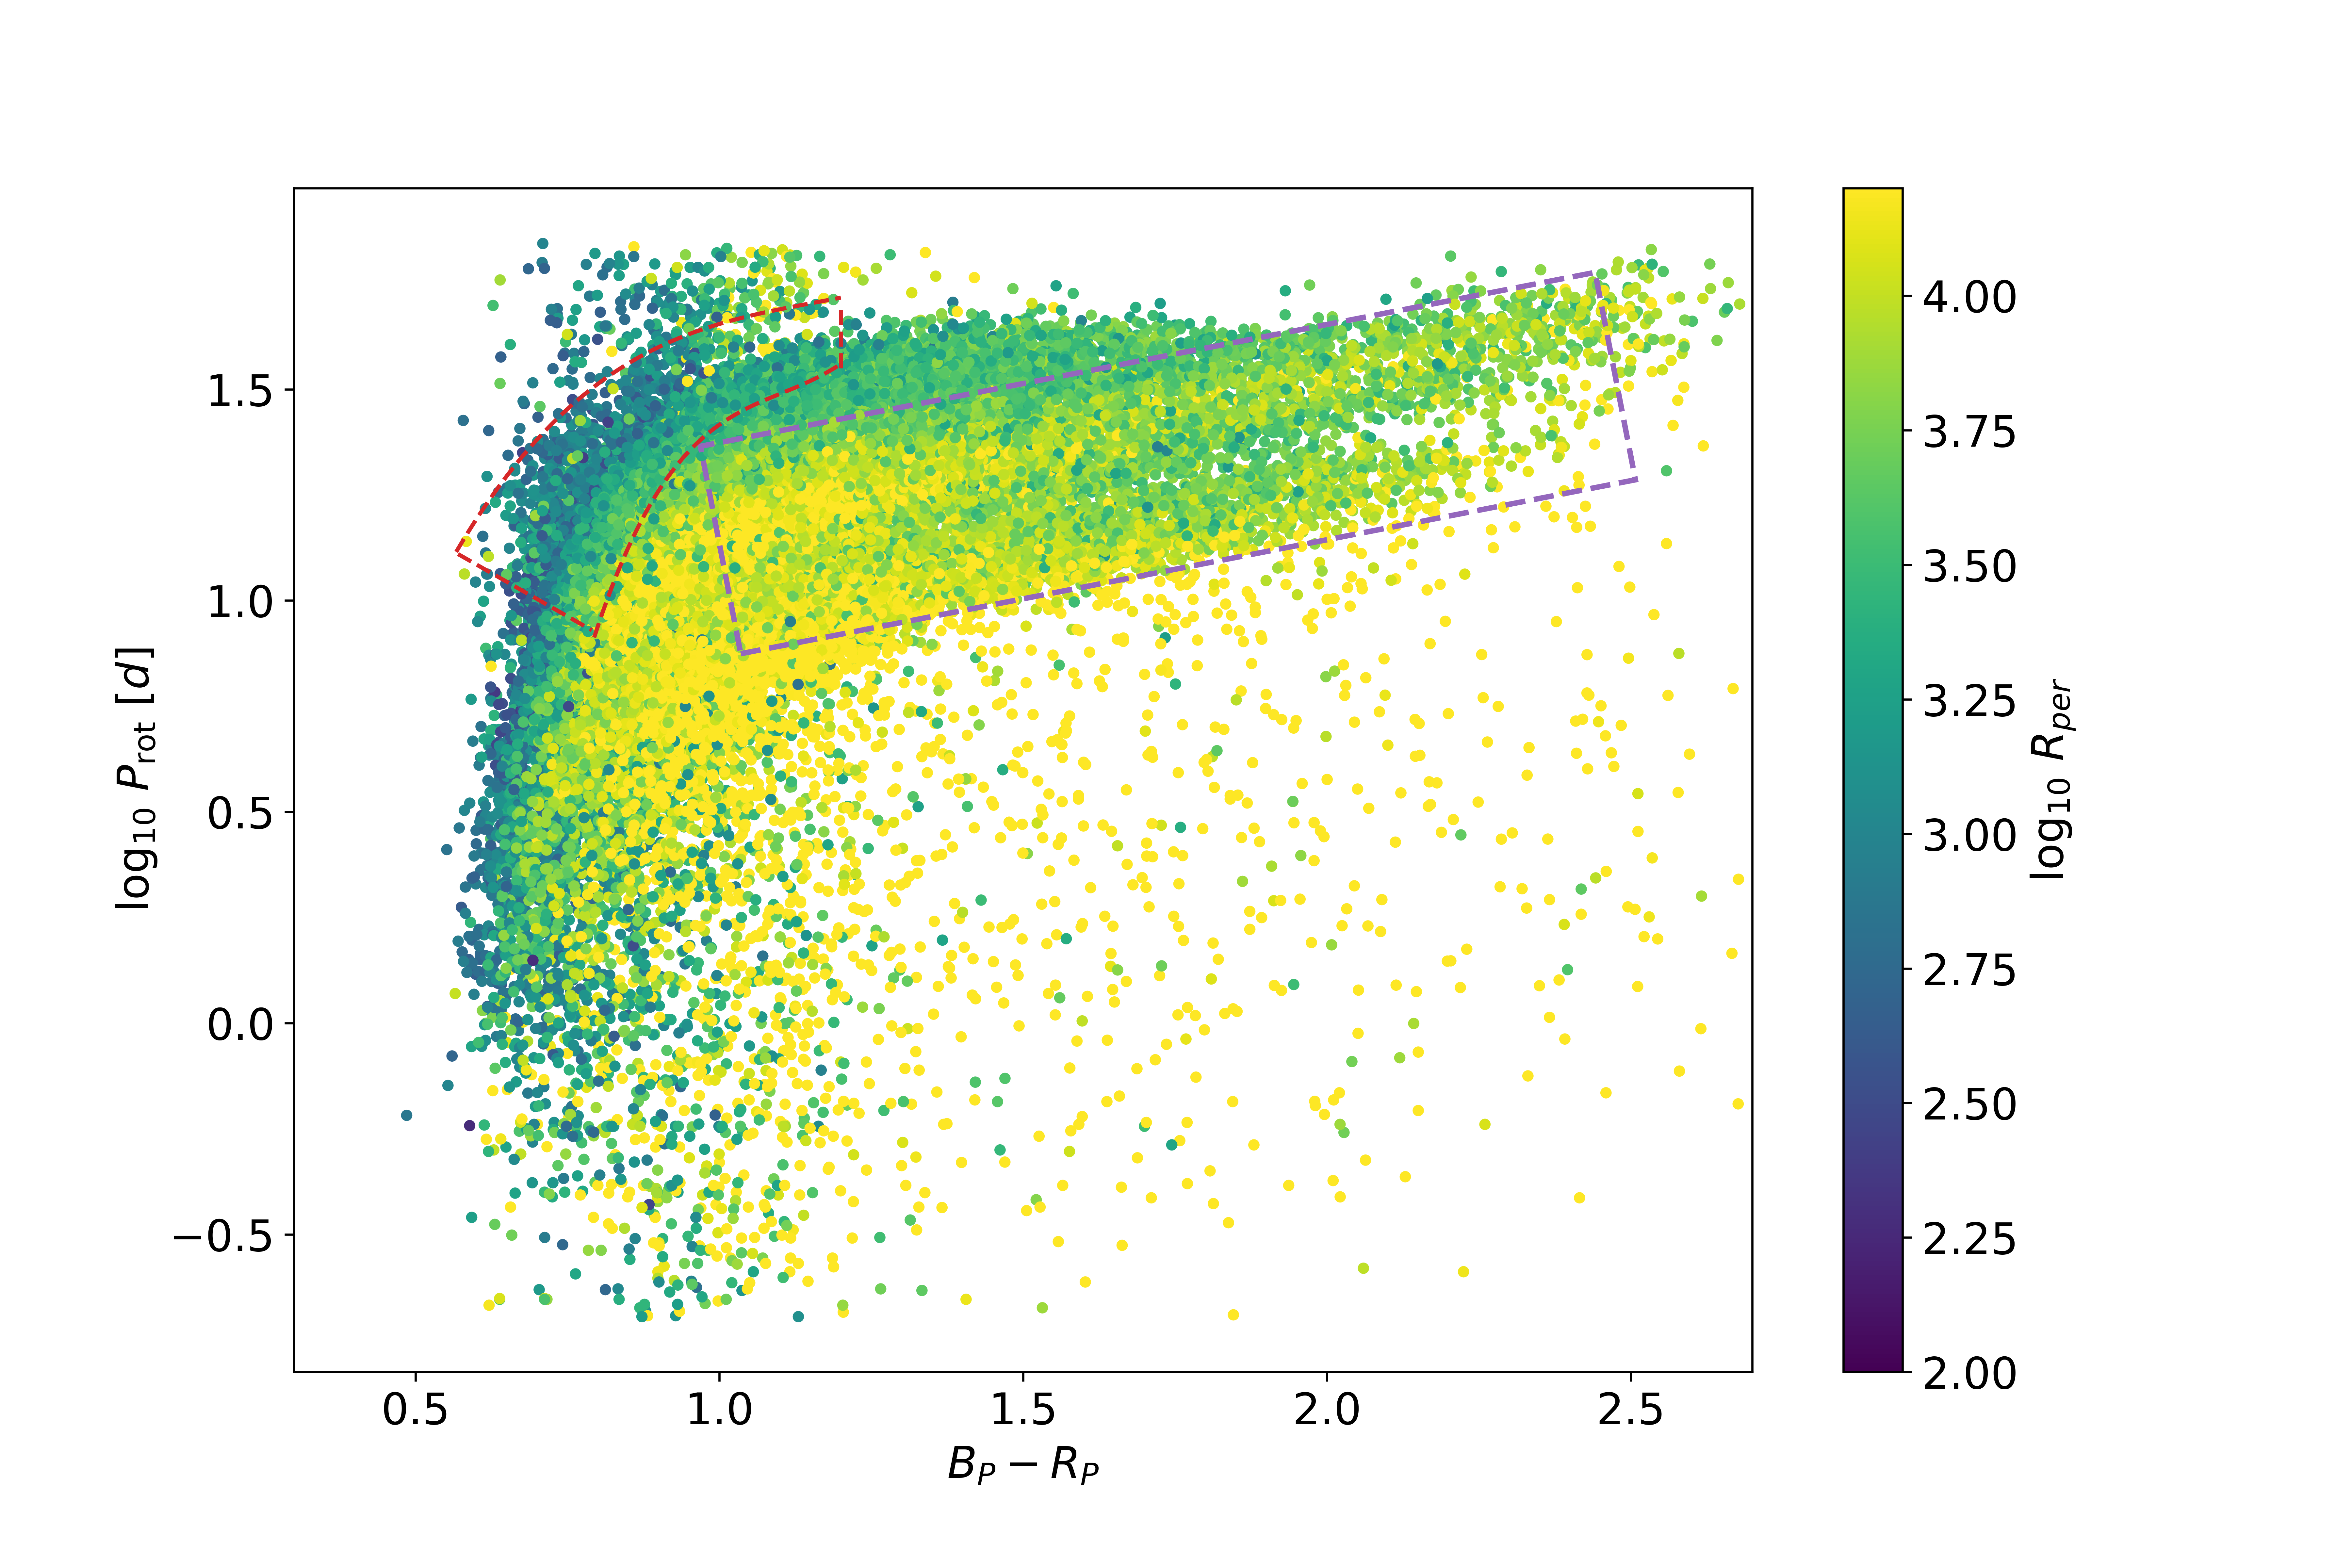
\includegraphics[width=\textwidth]{Figures/intro_figures/kepler_rot_dist.png}
    \caption{Scatter plot \gaia{} $B_P-R_P$ colour against log of the rotational period of the \kepler{} \citet{mcquillan_rotation_2014} rotational period sample coloured by the log of the photometric variation ($R_{var}$).
    $R_{var}$ decreased towards the gap from above and below, suggesting the intermediate period gap is representative of a minimum of observability of rotation period. Highlighted by arrows in this Figure are two features that we discuss in more detail in this Section: the intermediate period gap and the long-period pile-up.}
    \label{fig:kepler_rot_period}
\end{figure}

Since identifying the gap, several explanations have been presented for this phenomenon.
\citet{mcquillan_rotation_2014, davenport_rotating_2017} first proposed that rather than the gap being the result of modified angular momentum transport, the gap is the artifact of a recent period of bursty star formation in the \kepler{} field - resulting in a young ($<$ 50 Myr), fast rotating, population and older, background slowly rotating, population.
\citet{davenport_rotating_2017} further find that the fast and slow rotators in his sample also exhibit a different distribution of the proper motion.
Two kinematically separate groups favour the explanation of two epochs of star formation in the \kepler{} field. 
This explanation is further supported by the work of \citet{davenport_rotating_2018}, who showed that the gap appears to correlate with Galactic height, which is assumed to be related to stellar age.

The recent bursty star formation hypothesis accounts for the overpopulation of observations below the gap. 
In contrast, the dearth of observations represents the background observation rate of rotational periods within this period range.
\citet{gordon_stellar_2021} provided evidence against this hypothesis through analysis of \ktoo{} data.
They found that the intermediate period gap is present in the multiple pointings of the \ktoo{} mission - suggesting that recent bursty star formation is isotropic -  and that clusters with different ages contain stars that have crossed the gap.

The former suggests that all clusters universally went through a period of bursty star formation $\sim$50 Myr ago. 
\citet{angus_exploring_2020} observed that the velocity dispersions of stars increase smoothly across the gap.
Given that the two populations - above and below the gap - do not substantially differ in other spectroscopic and photometric observations, this scenario remains theoretically possible but unlikely.
The latter requires slightly more thought. Comparing Figures \ref{fig:cluster_rotational_periods} and of \ref{fig:kepler_rot_period}, the gap has a sharper slope than the sequences associated with constant age populations from Praesepe \citep{douglas_poking_2017,douglas_k2_2019}, NGC 6811 \citep{curtis_temporary_2019} and Ruprecht 147 \citep{curtis_when_2020}. 
If the bimodal star formation scenario explained the gap, the gap should have the same shape and position for each cluster and the entire \ktoo/\kepler{} sample.

Before exploring possible explanations for the intermediate period gap, it is worth identifying where the rotational period gap occurs in the stars' evolution.
\citet{reinhold_transition_2019} first suggested that the gap aligns with a rotational isochrone at $\sim$ 800Myr.
With \citet{spada_angular_2016} modifications to Skaumanich spin down for low-mass star to reflect the rotational distribution of clusters of known age, updated the proposed age to ~750 Myr \citep{reinhold_transition_2019}.
Contrary to the hypothesis that the gap aligns itself with a certain isochrone, \citet{curtis_when_2020} identified that the open cluster Ruprecht 147 contains stars above and below the gap - as well as one star that appeared to be within the gap.
This suggests that the gap does not align itself with a particular age.
Instead, they argued that the gap aligns itself with a line of constant Rossby number\footnote{Defined as the ratio of the rotational period to the convective turnover timescale ($Ro = P_{rot}/\tau_{conv}$) - which itself is dependent on mass and is approximately constant for a star's main-sequence lifetime} = 0.5.
The Rossby number is associated with the magnetic dynamo, e.g. \citet{noyes_rotation_1984, montesinos_new_2001, augustson_rossby_2019}
To simplify, a star can be thought of as a volume of charged particles.
As a star rotates, so do the charged particles within it.
Moving charged particles induce a magnetic field - creating a magnetic dynamo.
As the star rotationally evolves, so does the magnetic dynamo.

Given that the gap appears to line up with a line of constant Rossby number, this may suggest that the gap is instead caused by an event in the evolution of the magnetic dynamo rather than an event in time.
This is a notable result because the magnetic dynamo is associated with a number of stellar phenomena - such as magnetorotational instabilities (angular momentum transport processes associated with the magnetic field) or stellar spots.

Other prospective hypotheses for the intermediate period gap can be broken down into two categories: (1) modified angular momentum transport and (2) decreased observability of rotation periods.

Let us consider the first hypothesis: the gap results from modifications to angular momentum transport.
\citet{lu_bridging_2022} have shown that the gap is most apparent for stars less massive than 1.3 M$_{\odot}$ and more massive than 0.4 M$_{\odot}$.
If we look closely at Figure \ref{fig:ztf_comp} we can see that for the \ZTF{} sample (black dots) the intermediate period gap is most apparent for stars 1.5$<B_P-R_P <$2.5 and closes for low mass ($B_P-R_P >$2.5) stars.
Stars redder than $B_P-R_P >$2.5 are fully convective \citep{amard_first_2019}, suggesting that the gap may be another phenomenon related to the interplay between angular momentum transport between the radiative core and convective surface and surface rotational braking along the main sequence.

\begin{figure}[h]
    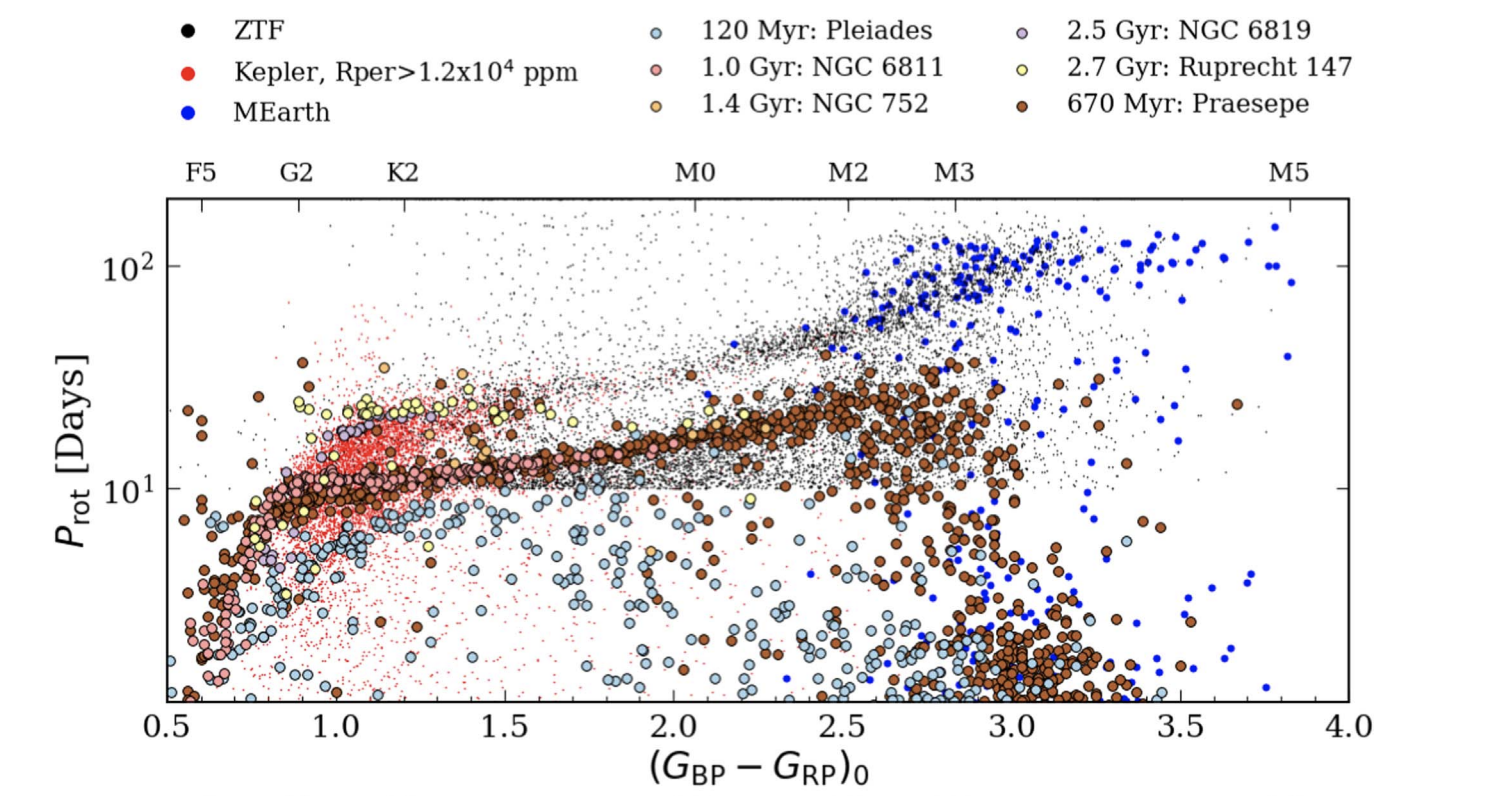
\includegraphics[width=\textwidth]{Figures/intro_figures/ztf_comp.png}
    \caption{Rotation period against \gaia{} $B_P - R_P$ from \kepler{}, \ZTF{} overlayed with various open cluster measurements. Highlighted by this Figure is the disappearance of the intermediate period gap above $B_P-R_P$ = 2.5 - the fully convective star boundary. This suggests that the rotational period gap is related to the coupling of the core and surface of low mass stars (0.4 $M_{\odot}<M<1.3M_{\odot}$). Sourced from the top panel of Figure 8 in \citep{lu_bridging_2022}.}
    \label{fig:ztf_comp}
\end{figure}

\citet{mcquillan_rotation_2014} first proposed that the gap is the result of two variations to Skaumanich rotational evolution.
First, stars below the gap undergo a period of stalled spindown, resulting in the observed overdensity of stars along the lower branch, followed by a period of accelerated spindown, resulting in the dearth of stars in the gap\footnote{The authors disfavoured the hypothesis favouring the bimodal star formation hypothesis discussed earlier in this work.}.

The proposed mechanism underlying this scenario is the mass-dependent decoupling and recoupling of the core and the envelope proposed in 
\citet{lanzafame_rotational_2015} and \citet{spada_competing_2020}, discussed earlier in this work.
\citet{angus_exploring_2020} suggest that the core envelope decoupling and recoupling may explain the period gap as a break between a "younger" pile-up regime (Ro$<$0.6) in which surface rotation periods are relatively constant with time from core-surface angular momentum transport and increase with decreasing mass from an "older" (Ro$>$0.6) regime with the gap representing a period of relatively fast spin evolution during the transition between the two.
Proponents of this hypothesis suggest that the gap results from a period of enhanced spindown following core and surface recoupling where stars "jump" the gap before resuming Skumanich spindown, as is observed for older clusters.
Models of - and physical mechanisms underlying - rotational evolution that reflect the proposed rapid spindown are yet to be identified.
Under this model, the gap reflects an under the density of stars but would not be empty.
There should be a small number of stars with Ro $\approx$ 0.6, irrespective of our ability to measure their rotational periods.
\citet{curtis_when_2020} found five Ruprecht 147 stars in or just beneath the gap yet to be thoroughly investigated.

Now let us discuss the second hypothesis: the gap results from a lack of observations of rotational periods.
The rotational period of \kepler{} stars requires that stars express photometric oscillations from stellar spots.
Starspots are regions of intense magnetic activity on a star's surface from magnetic flux tubes in the convection zone. 
These flux tubes are thought to be stretched and curled by the differential rotation of the convective region. 
As a result, convection is inhibited, limiting plasma flow to the surface in these tubes.
This results in lower-temperature material within the tube, which looks like a darker spot on the star's surface.
Stellar spots have bright perimeters surrounding the cooler internal regions of spots, known as faculae.

Stellar spots can both increase or decrease stars' bolometric luminosity.
 \citet{reinhold_fast_2013} and \citet{reinhold_transition_2019} propose that the gap represents the transition in stellar spot structure from spot to faculae dominance in the photosphere.
Following their explanation, the gap corresponds to a transition where the increase in bolometric luminosity from the faculae negates the decrease from the internal, cooler region of the stellar spots. 
In the \citet{mcquillan_rotation_2014} sample, stellar rotational periods are measured from the period of brightness variability due to the brightness variability introduced by stellar spots\footnote{this technique is discussed in more detail in Section \ref{sec:stellar_spot_brightness_modulations}}.
Suppose the bolometric flux does not vary due to stellar spots in the gap region. 
In that case, the amplitude of periodic variability would decrease within this region.
\citet{reinhold_transition_2019} suggests that the gap is full of stars and represents a minimum in the detectability of rotation periods.

Supporting this hypothesis, in both the \kepler{} and \ktoo{} fields, the variability amplitude ($R_{var}$) decreases towards the gap from both lower and higher rotational periods.
This can be seen in Figure \ref{fig:kepler_rot_period}, which is coloured by the log of $R_{var}$.
On the other hand, while there is evidence that stars undergo spot-to-faculae dominance, e.g. the Vaughan-Preston gap \citep{vaughan_survey_1980}, this occurs much later in a star's lifetime at Ro $\sim$ 1.
Further, there is evidence that stars above and below the gap are both spot-dominated  \citep{lockwood_patterns_2007, reinhold_transition_2019}.
\citet{reinhold_transition_2019} speculate that activity cycles that vary the spot-to-faculae brightness contributions on rotational timescales could be the process underlying the rotational period gap.
As of writing, there is no evidence to support this hypothesis.

Recent works have attempted to identify the fractional spot coverage of cluster members from their spectra \citep{cao_starspots_2022}.
They do this by assuming the spectra of stars can be broken down into spot and ambient components that vary in temperature but are consistent in other stellar parameters.
They find that the fractional spot coverage of stars is related to the Rossby number.
Within this work, they observe a population of spot-coverage-enhanced stars that deviate from the relations they present.

In a follow-up work \citep{cao_core-envelope_2023} they combine the angular momentum transport and decreased observation hypothesis by proposing
that star spot measurements in the Praesepe open cluster are strongly enhanced only for stars that depart Skumanich rotational evolution.
They suggest that a decoupling of the core and the surface explain both observations.
In their model, angular momentum transport between the core and the surface slows the increase of the rotational period. 
The resultant shears enhance the magnetic dynamo and, thus, stellar spot activity.
Stars enhanced in stellar spot coverage are expected to have decreased observed effective temperatures.
Spot-dominated, as opposed to faculae-dominated, stellar spots are cooler than the ambient temperature of the star.
As a result, stars with enhanced stellar spot coverage have a decreased observed effective temperature.
They then speculate that the rotational period gap is thus the result of a bias in observed effective temperature rather than a lack of observations of the rotational periods of stars in the gap.

Observations of open cluster rotational distributions beyond the gap suggest that stars $<1M_{\odot}$ that have crossed the gap (Ro$>$0.6) continue to spin down and follow the Skumanich-like rotational evolution until they leave the main sequence.
On the other hand, there is an apparent overabundance of stars at critical rotation periods (dependent on their mass). 
Above this is a lack of observations of rotation periods for stars $>$5500K.
Stars with higher masses also appear to have lower rotation periods on the pile-up than their less massive counterparts.
This results in what is known as the long-period pile-up, as noted in Figure \ref{fig:kepler_rot_period}.
The long-period pile-up aligns itself in the \citet{mcquillan_rotation_2014} period distribution with Rossby number  (Ro = 2.08) \citep{van_saders_forward_2019}.
 
\citet{van_saders_forward_2019} suggest that the long-period pile-up could result from decreased magnetic braking or a lack of observations of stars beyond this Rossby number.
Under the former scenario, stars stop spinning down when they reach this Rossby number as a result of weakened magnetic braking.
This results in the overdensity of stars and a lack of observations of larger rotational periods.
In the latter, they propose that the error in observed periods can smooth out the overdensity of stars and, infact the lack of rotational periods is because of variations to the stellar spot activity (See above discussion of speculative explanations for decreased observation of rotational periods within the rotational period gap).
Further supporting this explanation \citet{david_further_2022} found that photometric variability decreases above the gap.
Suggesting an unobserved population of stars with longer rotation periods.

Under the weakened magnetic braking model \citet{david_further_2022} suggest that stars in this temperature regime $1M_{\odot} < M < 1.3M_{\odot}$ may spend half of their main-sequence lifetimes at the long period pile-up with only modest variances to their rotational period.
Below this mass regime, stars appear to continue to lose angular momentum through wind braking following the Skumanich relation.
This results in stars with large rotational periods when they enter the post-main-sequence.

\subsection{Post-main-sequence}

For low mass (1.1 - 1.5 M$_{\odot}$) stars during the post-main-sequence, the information provided to angular momentum transport by each star can be greater than during the main sequence.
While surface rotation rate can still be measured through stellar spot photometric oscillations, within this regime, the core and surface can also be simultaneously constrained through asteroseismology (at different points in evolution). 
This results from a combination of the expression of mixed modes, shorter mode lifetimes, and increased core rotation rates.
During the main sequence, g-modes are trapped within the radiative core and thus do not introduce brightness variations (oscillations) to the stellar surface.
Some g-modes can couple with p-modes in the surface convective cavity during the post-main-sequence and are known as "mixed modes".
The rotational splittings of the mixed modes allow us to infer the rotation rate in the radiative region and deep core. \citep{metcalfe_precise_2010,bedding_gravity_2011}
Where, precisely, the mixed modes probe is dependent on where in the post-main-sequence the star is observed.
For example, sub-giant stars express p-modes and mixed modes that can probe both the core and the surface, whereas red giant branch (RGB) stars mainly express mixed modes that can only probe the star's core.
While stellar spot surface rotation periods can be measured for post-main-sequence stars \citet{mcquillan_rotation_2014, ceillier_surface_2017}, asteroseimic inference of core and surface rates is the standard for probing rotation evolution in this evolutionary regime \citep{deheuvels_seismic_2014, gehan_core_2018, deheuvels_seismic_2020, fellay_asteroseismology_2021}.

Measuring the core and surface rotation rates simultaneously provides much more information to angular momentum transport than either of these quantities alone.
For example, during the main-sequence, the over-abundance of stars along the lower branch of the Kepler rotation period gap could simultaneously be explained by diminished wind braking for the surface or by core-envelope recoupling.
Measuring the core rotation rates would break this degeneracy.
This asteroseismic quirk is useful as it allows us to directly investigate angular momentum transport more efficiently.

However, the constraints to the rotation profile of stars by asteroseismology, even in the post-main sequence, are limited.
Indeed the core and surface rotation rates of subgiants can simultaneously be probed.
However, where in a star the rotation can be probed depends on the observed oscillation modes, which depend on the stellar structure.
The rotation rates obtained by asteroseismology are kernel-based averages of the rotation profile in regions that the observed oscillation modes probe.
For example, subgiants' core and surface rotation rates are the kernel-based average rotation rates of the innermost $r/R$<0.05 and outermost $r/R>0.9$ regions (on average).
Between these regions, the rotation profile is not constrained.
As a result, the shape of the rotation profile, which can be fingerprints of specific angular momentum transport mechanisms at play, is also not constrained.

Asteroseismic inference of rotation rates can also be imprecise.
This can be seen when comparing the surface rotation periods from asteroseismology and stellar spot photometric oscillations in \citet{hall_weakened_2021}.
This is because: a) state-of-the-art measurements of rotational splittings - the quantity that constrains the rotation profile - are low SNR and are often also imprecise, and b) the observed rotational splittings are a finite subset of the infinite number of rotational splittings that would be required to accurately and precisely constrain the entire rotation profile.
With these limitations in mind, we now discuss the observed evolution of rotation of post-main-sequence stars.

Following the main-sequence, low-mass stellar rotation varies with the evolutionary phase.
Models of rotating stellar evolution (e.g. )\citep{maeder_evolution_2000,heger_2000} predict the following qualitative evolutionary pathway.
Towards the end of the main sequence the rotation profile is largely flat.
Assuming conservation of angular momentum as hydrogen core burning stops, pressure in the core drops, resulting in core contraction while the convective surface region expands.
Resultingly the core is spun-up while the surface is spun-down.
The core should continue to spin down as the core contracts along the RGB until entering the red clump (low-mass core He burning).
The core burning reintroduces core pressure, and the resulting expansion of the core decreases the core rotation rate.
When core He burning ceases, the core pressure drops again, resulting in a spun-up white dwarf (relative to the core rotation rate of red clump stars).
We highlight the qualitative rotation evolution of post-main-sequence stars in Figure \ref{fig:poms_evo}.
Observations suggest that low-mass stars follow this pathway \citep{mosser_spin_2012,deheuvels_seismic_2014,deheuvels_seismic_2015,hermes_white_2017,gehan_core_2018,deheuvels_seismic_2020}.

\begin{figure}[h]
    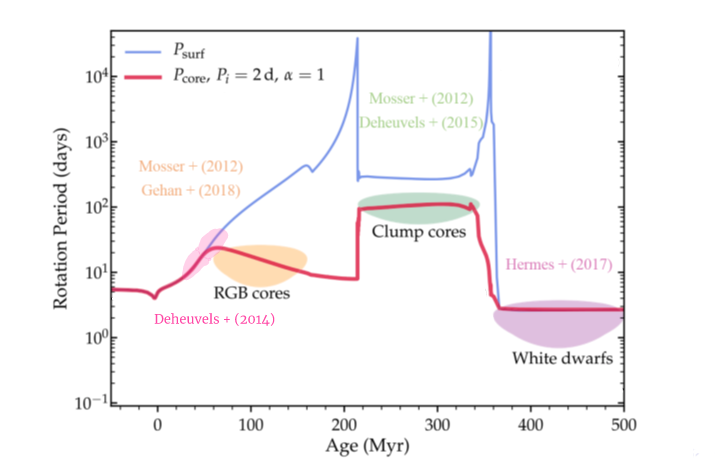
\includegraphics[width=\textwidth]{Figures/intro_figures/qualitative_evo.png}
    \caption{Core (red) and surface (blue) rotation rates with additional angular momentum transport following the prescription of \citet{spada_angular_2016}. Coloured sections denote evolutionary milestones and the works that have provided constraints to these milestones. \textbf{Pink:} subgiant core and surface rotation, \textbf{Orange:} red giant branch cores, \textbf{Green:} clump core rotation rates, and \textbf{Purple:} white dwarf rotation rates. Adapted from Figure 3 in \citet{fuller_slowing_2019}}
    \label{fig:poms_evo}
\end{figure}


Measuring the core and the surface rotation rates of post-main-sequence stars allows us to place constraints on the radial differential rotation of stellar interiors and quantitatively probe the evolution of angular momentum transport.
Observations of young subgiants suggest that terminal age main sequence stars' rotation profiles are relatively flat \citep{deheuvels_seismic_2020}.
However, observations of older post-main-sequence stars have raised more questions than they have answered \citep{beck_fast_2012}.
To summarise: angular momentum transport during the post-main-sequence must be greater than state-of-the-art models currently predict.

\citet{deheuvels_seismic_2014} measured the core and surface rotation rates of 6 subgiants/young red giants.
The observed core to surface rotation ratio of subgiants and the core rotation rates of red giant branch stars suggest that additional angular momentum transport is unaccounted for in state-of-the-art models of rotating stellar evolution \citep{deheuvels_seismic_2014, spada_angular_2016, moyano_asteroseismology_2022}.
The scale of the core-to-surface rotation rate ratio of subgiants ($\Omega_c/\Omega_s$) is one to two orders of magnitude smaller than models predict \citep{fuller_asteroseismology_2015,spada_angular_2016,ouazzani_gamma_2018, eggenberger_asteroseismology_2019}.
While core rotation rates were first believed to decrease along the red giant branch\footnote{Indeed when core rotation rates of red giants are plotted against $\log{g}$, a proxy for evolution, they do appear to decrease with evolution. When plotted against the more appropriate scale of mixed mode coupling (See Equation 10 in \citet{gehan_core_2018} and compare Figures 12 and 13 in this work), they are constant with evolution.} \citep{mosser_spin_2012} revised measurements and a larger sample size revealed that the core rotation rates of red giant branch stars appear constant with evolution when the contraction of the core should spin them up.
\citep{mosser_spin_2012,gehan_core_2018,moyano_asteroseismology_2022}.
The core rotation rates of early red giant branch and red clump stars suggest a continued excess angular momentum transport during this phase of evolution \citep{cantiello_angular_2014,moyano_asteroseismology_2022}.
On the other hand, observed white dwarf rotation rates can be recovered from the observed core rotation of clump stars assuming conservation of angular momentum. \citep{cantiello_angular_2014, den_hartogh_constraining_2019}
\citet{cantiello_angular_2014} suggests that this feature may be owing to the short evolutionary timescale between the red clump and white dwarf phases rather than indicative of a decrease in the excess angular momentum transport.


The physical mechanism underlying the excess angular momentum transport is currently unidentified.
Several notable relations with mass and evolutionary state have been determined by calculating the excess angular momentum transport required to match observations. 
\citet{spada_angular_2016} quantified the increased angular momentum transport required to match the observed subgiant core and surface rotation rates measured in \citet{deheuvels_seismic_2014}.
They introduced an additive angular momentum diffusion coefficient to the transport of angular momentum equation in the radiative zone, which obeys an advection-diffusion equation: 
\begin{equation}
    \rho \frac{\text{d}}{\text{dt}}\left(r^2 \Omega \left( r \right)\right) = \frac{1}{5r^2}\frac{\partial}{\partial r}\left(\rho r^4 \Omega \left( r \right)
 \ U\left(r\right)\right) + \frac{1}{r^2}\frac{\partial}{\partial r} \left(\rho \left( D_{\text{shear}} + v_{\text{add}}\right) r^4 \frac{\partial \Omega\left( r \right)}{\partial r}\right),
\end{equation}
\citep{zahn_circulation_1992,maeder_stellar_1998,eggenberger_geneva_2008}
where $r$ and $\rho$ are the characteristic radius and density on an isobar. $\Omega(r)$ is the mean rotational rate and $U(r)$ is the velocity of meridional currents in the radial direction. $D_{\text{shear}}$ is the diffusion coefficient for the angular momentum shear instability (See Equation 10 in \citet{eggenberger_effects_2010}) and $v_{\text{add}}$ is the additional viscosity corresponding to the excess angular momentum transport.
Their results suggest that the additional angular momentum transport decreases as stars ascend the subgiant branch and increases with mass.
The suggested scale of excess angular momentum transport they propose is on the order of $10^3-10^4 \text{cm}^2 \text{s}^{-1}$.
Which is similar to $D_{\text{shear}}$ close to the convective envelope but rapidly decreases to the order of $10^1\text{cm}^2 \text{s}^{-1}$ in the stellar core.
Comparing Figures \ref{fig:deh_without} and \ref{fig:deh_with} we see that the introduction of the additional viscosity to the model term results agreement with the core to surface rotation fraction in the \citet{deheuvels_seismic_2014} sample.

\citet{moyano_asteroseismology_2022} performed a similar analysis but with the core rotation rates of red giant branch and red clump stars measured in \citep{mosser_spin_2012} and \citet{gehan_core_2018}.
They found that the same order of magnitude additional viscosity term was required to explain the approximately constant core rotation rates of red giant and red clump stars.  
Qualitatively they found that the additional angular momentum transport becomes stronger when the star evolves up the red giant branch through shell hydrogen burning.
Angular momentum must be redistributed between two to three orders of
magnitude more efficiently for red clump stars than for red giants closer to the main-sequence turn-off consistent with \citet{den_hartogh_constraining_2019}.
Figures \ref{fig:rgb_cores_without} and \ref{fig:deh_with} highlight that models of red-giant evolution with the additional viscosity introduced in this work now agree with the observed core rotation rates observed in \citet{gehan_core_2018}.

\begin{figure}[h]
    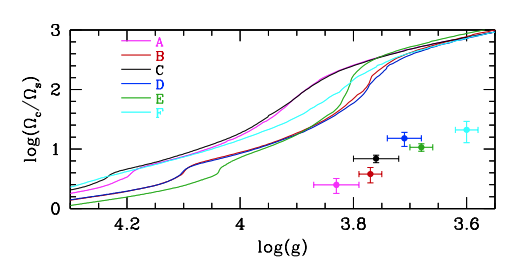
\includegraphics[width=\textwidth]{Figures/intro_figures/deheuvels_disparity_without.png}
    \caption{log of core to surface rotation rate against $\log{g}$. 
    \textbf{Dots:} Observed core to surface rotation rates of the six subgiants measured in the \citet{deheuvels_seismic_2014} sample (A,B,C,D,E,F).
    \textbf{Lines:} rotating models of the stars in that sample without additional angular momentum transport \citep{eggenberger_asteroseismology_2019}.
    The observed core-to-surface rotation rates are much smaller than models predict. This implies additional angular momentum transport than is currently accounted for models.
    Sourced from Figure 2 in \citep{eggenberger_asteroseismology_2019}.}
    \label{fig:deh_without}
\end{figure}

\begin{figure}[h]
    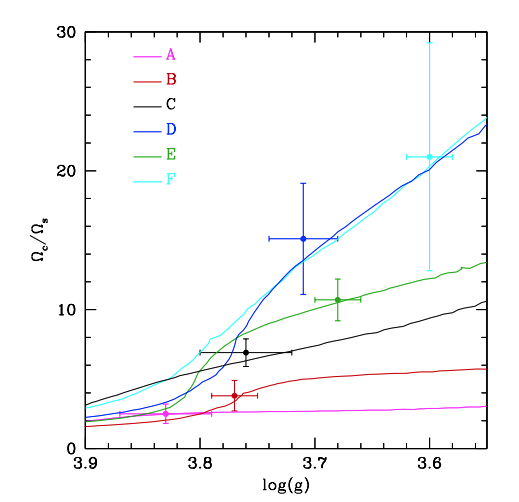
\includegraphics[width=\textwidth]{Figures/intro_figures/deheuvels_disparity_with.png}
    \caption{Same as Figure \ref{fig:deh_without} but with additional angular momentum transport introduced for the models to reflect the observations.
    Sourced from Figure 3 in \citep{eggenberger_asteroseismology_2019}.}
    \label{fig:deh_with}
\end{figure}


\begin{figure}[h]
    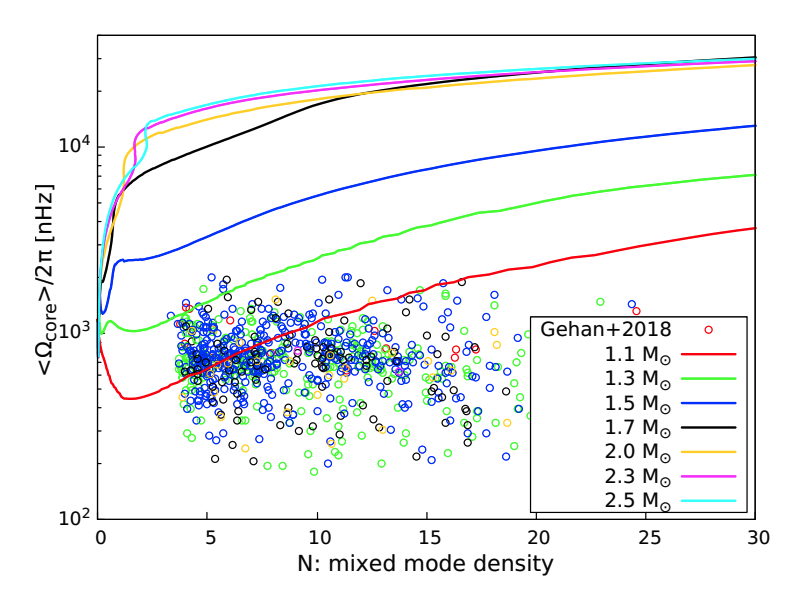
\includegraphics[width=\textwidth]{Figures/intro_figures/rgb_core_rot_without.png}
    \caption{Average core rotation rates of red giants against mixed mode density (a proxy for evolution) 
    \textbf{Dots:} Observed core rotation rates from \citet{gehan_core_2018}
    \textbf{Lines:} rotating models of the stars in that sample without additional angular momentum transport \citep{moyano_asteroseismology_2022}.
    The observed core rates are much smaller than models predict. Implying excess angular momentum transport is required for the models to reflect the observations.
    Sourced from Figure 6 in \citep{moyano_asteroseismology_2022}.}
    \label{fig:rgb_cores_without}
\end{figure}

\begin{figure}[h]
    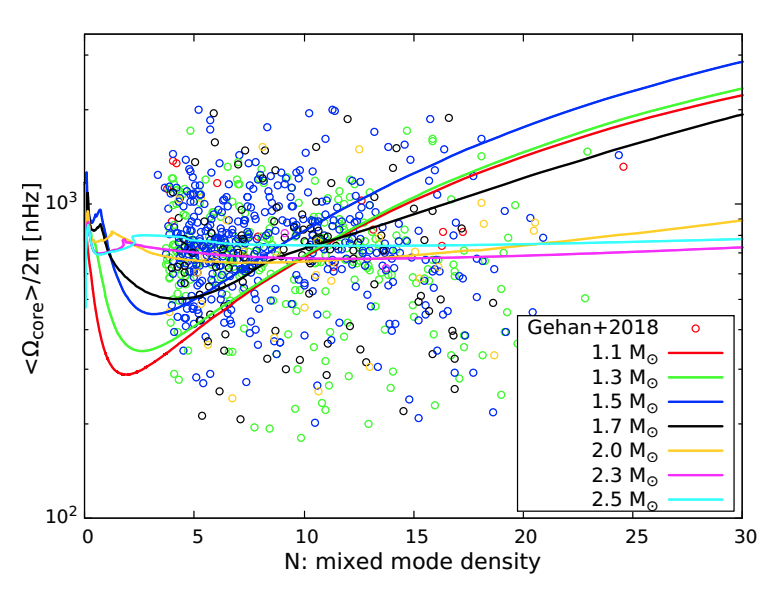
\includegraphics[width=\textwidth]{Figures/intro_figures/rgb_core_rot.png}
    \caption{Same as Figure \ref{fig:rgb_cores_without} but with additional angular momentum transport introduced for the models to reflect the observations.
    Sourced from Figure 7 in \citep{moyano_asteroseismology_2022}.}
    \label{fig:rgb_cores_with}
\end{figure}


Several modes of excess angular momentum transport have been suggested to explain the disparity between models and observations.
\citet{barker_angular_2019,barker_angular_2020} studied the role of
the Goldreich-Schuber-Fricke (GSF) instability (\citep{goldreich_differential_1967,fricke_rotation_1967} and its role in angular momentum transport for post-main-sequence stars.
They suggest that the GSF instability can introduce additional viscosity up to $10^4 \text{cm}^2 \text{s}^{-1}$ for low-mass stars but is two orders of magnitude too small to reflect the rotation of higher mass stars not discussed in this work.

Magnetorotational instabilities constitute another candidate to explain the internal rotation of evolved stars.
Two potential candidates are azimuthal magnetic rotational instabilities (AMRI) \citep{ruediger_astrophysical_2014,rudiger_diffusive_2015} and the Tayler-Spruit instability \citep{spruit_dynamo_2002} (See Section \ref{sec:magneto_rotational_instabilities}).
\citet{rudiger_diffusive_2015} suggest AMRIs can increase molecular viscosity to the magnitude required to explain observations.
On the other hand, there is no evidence to suggest that this instability reflects the trends with mass and evolution.
The Tayler instability does introduce excess angular momentum transport in the post-main-sequence \citep{fuller_slowing_2019}, however, it cannot simultaneously reflect the observations of both subgiants and red giants \citep{eggenberger_asteroseismology_2019,den_hartogh_constraining_2019}.


\citet{spada_angular_2016} propose the efficiency of angular momentum transport may be related to the core to surface rotation rate to some power - $\left(\Omega_c/\Omega_s\right)^{\alpha}$ - which can be related to magnetorotational instabilities.
This work suggests that $\alpha = 3$ reflects the core rotation rates of red giants claimed in \citep{mosser_spin_2012}.
\citet{moyano_asteroseismology_2022} revisited this prescription and found that $alpha = 3$ more accurately reflects the approximately constant rotation core rotation rates of red giants observed by \citet{gehan_core_2018}.
\citet{spada_angular_2016} was limited to a single model with mass = 1.25 $M_{\odot}$.
No parameterisation with mass was therefore performed.

Other physical mechanisms have been suggested to have a role in excess angular momentum transport, such as angular momentum transport by internal gravity waves \citep{pincon_can_2017} or mixed-modes \citep{belkacem_angular_2015}. 
However, the scale of their introduced additional viscosity is yet to be investigated.
Disentangling each of these proposed mechanisms' relative importance to the additional angular momentum transport required to explain the observations requires much more data.


%On the other hand the subgiant phase is short-lived and steroseismic inference of the rotation profile is data-intensive in that it requires short-cadence observations of stars over long observation periods for high enough SNR to measure rotational splittings.
%As a result, only ~30 subgiant and young red giants that exhibit oscillation modes that probe both the core and the surface have been asteroseismically probed.

We speculate that the simultaneous measurement of subgiants' core and surface rotation rates may be the best probes for constraining the excess angular momentum transport.
A few pathways exist to further probe the mechanism underlying excess angular momentum transport through asteroseismology alone.
Either: a) more stars need to have their core and surface rotation rates measured through asteroseismology (which we will denote ensemble fitting), or b) stronger constraints must be placed on the rotation profile between the core and the surface (single star constraints).

On the former, if more stars have their core and surface rotation rates observed, then more measurements of the excess angular momentum transport required for state-of-the-art models to match the observations are made.
The excess angular momentum transport required to match observations appears mass and evolutionary-dependent.
Stronger constraints to the dependency of the excess angular momentum transport on these quantities provide information about the underlying mechanism.
The Kepler asteroseismic data currently available suggests that the efficiency of the excess angular momentum transport increases with the star's mass \citep{eggenberger_asteroseismology_2019}.
However, the efficiency of angular momentum transport decreases with evolution during the subgiant phase.
Consequently, a transport process with efficiency dependent on the angular momentum gradient between the core and the surface cannot be at play in subgiants.
Identifying with more precision the dependency of excess angular momentum transport on stellar quantities would provide evidence for or discredit proposed mechanisms.

On the latter, the internal shape of the rotation profile of subgiants reflects the underlying mechanism that created it.
Therefore, evidence for or against particular shape of rotation profiles is illuminating to proposed mechanisms.
A strong gradient in the rotation profile in the core of a subgiant, for example, is incompatible with angular momentum transport through deep fossil magnetic fields \citep{gough_effect_1990} as they would likely smooth out sharp features.
 This is because differential rotation is expected to be damped along poloidal field lines (\citealp{garaud_rotationally_2002, strugarek_magnetic_2011}).
 Internal gravity waves, on the other hand, are expected to be efficient during the advanced phases of stellar evolution \citep{charbonnel_deep_2008}. 
Internal gravity waves can give birth to localised weak gradients in the rotation profile as a result of extraction and deposit of angular momentum \citep{charbonnel_influence_2005}. 
A sharp rotational gradient could also potentially trigger magneto-rotational instabilities that would transport angular momentum (\citealp{balbus_stability_1994,arlt_differential_2003,menou_magnetorotational_2006, fuller_asteroseismology_2015, fuller_slowing_2019,moyano_asteroseismology_2022}). 
Evidence of a strong angular momentum gradient towards the core of a sub-giants quickly constrains the number of possible angular momentum transport mechanisms to solve the angular momentum transport problem.

Two obvious problems impede the single-star pathway. 
These are the need for observations of high SNR higher degree modes and the results of methods used to measure rotation profiles being unstable to high-resolution inversions. 
Constraints on the rotation profile in intermediate points between the core and surface require the observations of oscillation modes of $l \approx 10$ \citep{ahlborn_asteroseismic_2020}. 
For reliable measurements of such oscillations, much longer observation periods, longer than \corot{} and \kepler{}, of sub-giants are required.
   
Both of these pathways require much more asteroseismic data than is currently available.
For ensemble fitting to be viable many subgiants would need to be observed over long baselines with short cadence observations.
If the Kepler mission is exemplary, then the baseline required for high-SNR asteroseismic observations is on the order of ~4 years per star.

At the time of writing, ~30 subgiants show evidence of rotational splittings \citep{li_asteroseismology_2020,li_asteroseismology_2020-1}, though the rotational splitting data is yet to be released and analysed.
The results will be undoubtedly informative, though we will not speculate exactly how much they will solve the subgiant excess angular momentum transport problem.
\citet{hatt_catalogue_2023} suggests that there is $\sim$4000 stars in the TESS - short cadence catalogue with observable solar-like oscillation features.
The measured frequency of peak oscillation power $\nu_{\text{max}}$ of stars in these sample suggests that some of these stars are subgiants.
While no rotational splittings of these stars have been reported some of these stars may lay in the continuous viewing zone.
This means their observation periods are approaching 4 years at time of writing and these stars may soon offer a seperate sample of subgiants with observations of asteroseismic rotational splittings.
While we may speculate about future asteroseismic focussed missions, it will be some time before any new asteroseismic rotation signals in subgiants are made.

Independent constraints can also be placed on the evolution of the surface rotation of subgiants.
\citet{santos_surface_2021} measured the surface rotation of 4500 subgiants using photometric oscillations from stellar spots.
The measured rotational periods against their effective temperature are shown in Figure \ref{fig:subgiant_surface}.
Within this Figure, there are a few notable features.
While subgiants are definitionally older than their main-sequence counterparts, there is a sample of fast-rotating stars coincident with the fast rotators on the main sequence.
This could be explained by most of the stars in this sample being a higher mass than the Kraft break.
They have passed through the main sequence with fast rotating surfaces, entering the subgiant phase; their effective temperatures decrease and are shifted to the right in this diagram relative to their main-sequence counterparts.
The high density of fast-rotating stars could also result from an observational bias.
Long rotational periods require longer baselines to recover and thus have a decreased observed fraction.
Among the sample is a group of slow-rotating (Period $>$ 60 days) targets with Teff between 5000 and 6000 K.
These are consistent with more evolved subgiants as the slowest of these targets are located close to the red giant branch.
This work also suggests that the decreased observation of rotation periods $>$60 days, the strong upper edge of the \citet{mcquillan_rotation_2014} rotational period distribution, is the result of a lack of observations of main-sequence stars rather than an inherent lack of long period probing power by \kepler. 
Whether the upper edge results from angular momentum transport or decreased photometric variability is unknown.
The final feature that is not commented on in their work is an apparent dearth of observations coincident with the intermediate period gap.
Whether this is real or a result of noise is an interesting avenue of research in further understanding the underlying mechanism of the intermediate period gap for main sequence stars.

\begin{figure}[h]
    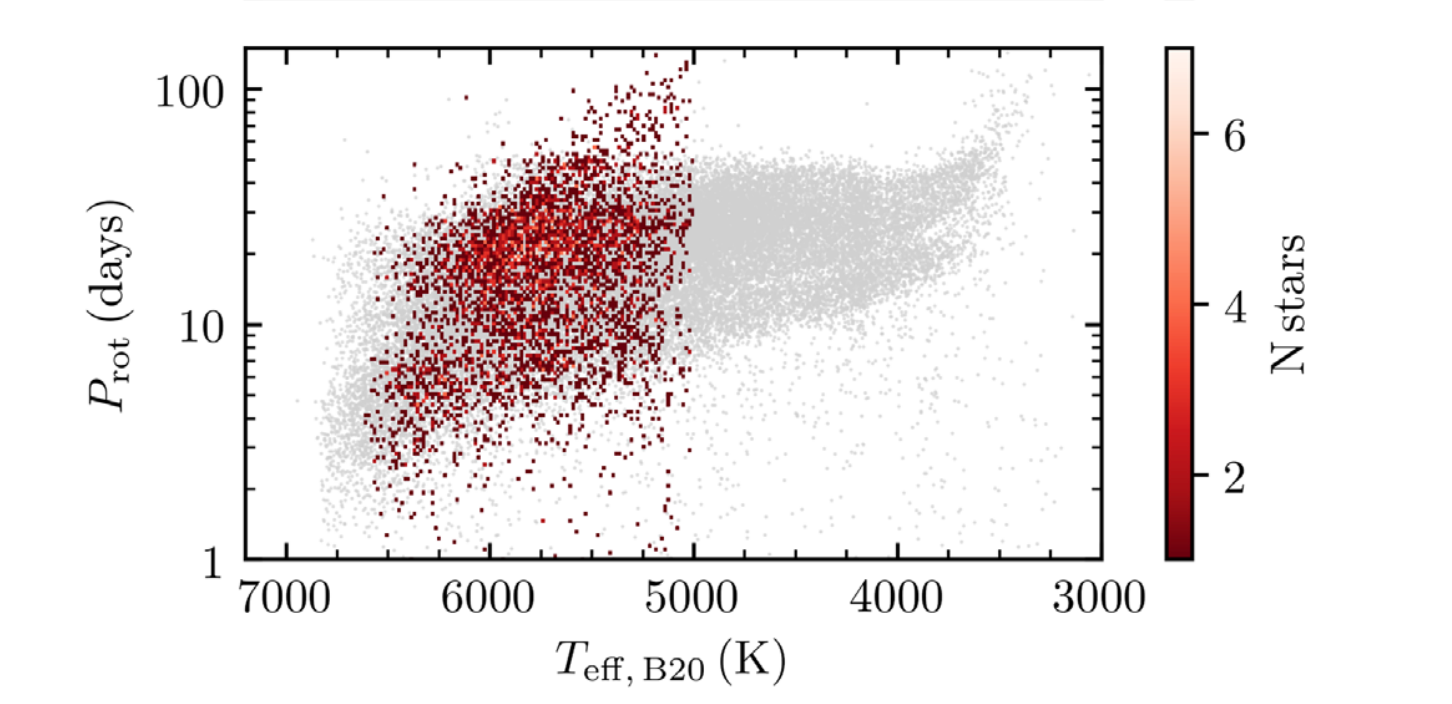
\includegraphics[width=\textwidth]{Figures/intro_figures/subgiant_surface.png}
    \caption{Surface rotation period against effective temperature of subgiants in the \citet{santos_surface_2021} sample overlayed over the \kepler{} \citet{mcquillan_rotation_2014} sample. 
    Sourced from the bottom panel of Figure 5 in \citep{santos_surface_2021}.}
    \label{fig:subgiant_surface}
\end{figure}

\citet{ceillier_surface_2017} measured the surface rotation periods of 361 red giants from stellar spot photometric variability.
The measured rotational periods against their mass are shown in Figure \ref{fig:rgb_surface}.
Expectedly, comparative to the subgiant analysis of \citet{santos_surface_2021} the surface rotation period of red giant stars is greater than their subgiant counterparts.
They suggest that the surfaces of these stars rotate faster than models suggest \citep{tayar_rapid_2015}.
They conclude that the large percentage of rapid rotators must result from interactions of red giants with other bodies.
This work, however, is older than the revised excess angular momentum transport research discussed earlier in this work.
Their results need to be reexamined within the context of excess angular momentum transport.

\begin{figure}[h]
    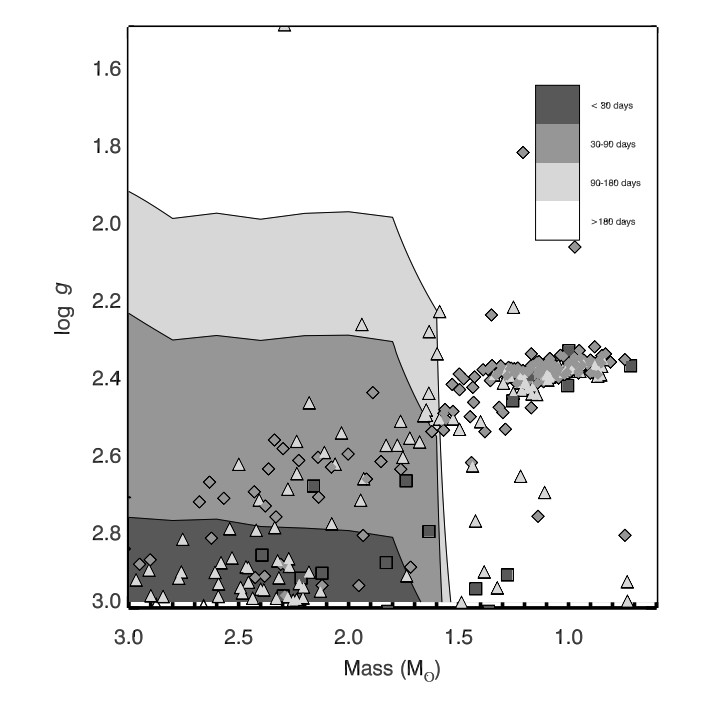
\includegraphics[width=\textwidth]{Figures/intro_figures/rgb_surface.png}
    \caption{Surface rotation period against mass of red giant stars from \citet{ceillier_surface_2017}.
    Sourced from the top panel of Figure 7 in \citep{ceillier_surface_2017}.}
    \label{fig:rgb_surface}
\end{figure}

Finally, we discuss the rotating remnants of low-mass post-main-sequence evolution: white dwarfs.
White dwarfs do not evolve rotationally, though their observed rotation rates constrain angular momentum during the red clump phase.
\citet{hermes_white_2017} suggest that the rotation periods of white dwarfs decrease with the progenitor's mass.
As previously discussed, the surface rotation rates of white dwarfs are consistent with angular momentum conservation following the red clump \citep{den_hartogh_constraining_2019, cantiello_angular_2014}.
This is because the time scale of angular momentum transport is longer than the timescale of evolution from red clump star to a white dwarf.
\citet{den_hartogh_constraining_2019} suggest that mass-dependent angular momentum transport must decrease with evolution along the red clump such that the angular momentum of terminal red clump rotation cores agree with the angular momentum of white dwarf stars.

\section{Effects of rotation}
\label{sec:effects}

Within the previous Section, we discussed the evolution of rotation from birth to remnants of evolution.
While we now have an understanding of this evolution, we still need to clarify the effects of rotation on stellar evolution.

\subsection{Hydrostatic effects}

The effects of rotation on stellar evolution are varied and complex.
In general, the hydrostatic effects of rotation have only minimal effects on the internal evolution of stars \citep{kippenhahn_rotation_1970,maeder_evolution_2000}.
Especially the low-mass, slowly rotating stars we consider in this work.
In this Section, we review how some of these effects are treated in current models of stellar evolution, the resulting changes to stellar evolution brought about by these effects and their observable consequences.
We will begin by discussing the effects of stellar rotation on hydrostatic equilibrium.


As a star rotates, its equilibrium configuration deviates from the non-rotating hydrostatic equilibrium due to centrifugal forces. 
Rotation-induced centrifugal forces induce deviations from spherical symmetry.
Only if the rotation energy of a star approaches a significant fraction of the gravitational potential energy will observable triaxial deformation occurs.
Low-mass stars usually rotate slowly, so these effects are rarely seen.

The four equations of stellar structure need to account for this change to the equilibrium configuration.
\citet{kippenhahn_simple_1970} devised the method to account for this where a conservative potential exists.
In this method, they replace the notion of spherical stratification of non-rotating stars with a rotationally deformed shellular stratification where the structural variables - e.g. pressure ($P$), density ($\rho$), temperature ($T$), chemical abundances - are constant on an equipotential.
The equipotential in this prescription is defined as 
$\Psi = \Phi + \frac{1}{2}\Omega^2 r^2 \sin^2 \theta$, the non-rotating gravitational potential modulated by the centrifugal force, where $Phi$ is the gravitational potential, $\theta$ the latitude relative to the rotational axis and $\Omega$ the angular rotation rate.
This method applies only when a conservative potential exists, i.e. when the angular velocity distribution is cylindrically symmetric \citep{tassoul_theory_1978}.
The internal rotation generally evolves towards rotation laws that are non-conservative.
For example, \citet{zahn_circulation_1992} suggests that turbulence is anisotropic, with a stronger transport horizontally than vertically. 
This results in a constant rotation rate on isobars and does not fall into the conservative case.
\citet{maeder_diffuse_1996} revise \citet{kippenhahn_circulation_1974}'s method and prescribe a consistent description of shellular rotation on isobars which is valid for slow rotation.
On these isobars, the non-rotating stellar variables and angular momentum are constant. 
This allows models of rotating stellar evolution to be kept one-dimensional.

The equations of stellar structure are mainly affected by rotation through a few key concepts.
Centrifugal forces reduce effective gravity for all points in the star that are not on the axis of rotation.
The centrifugal forces vary with radial distance and latitude, resulting in equipotentials closer together along the rotational axis than the equatorial axis.
Radiative flux varies with local effective gravity \citep{von_zeipel_radiative_1924}.
This results in gravitational darkening \citep{von_zeipel_radiative_1924, kippenhahn_rotational_1977} - stars are higher temperature and have larger temperature and radiation flux along the rotational axis compared to the equatorial axis.
Gravity darkening of slowly rotating stars (rotation rates much slower than the break-up velocity like those considered in this work) is very small - $<<$0.1\% variation in luminosity and temperature across their surfaces.
Stars close to critical rotation rate should be treated with care \citep{kippenhahn_rotational_1977,maeder_stellar_1999,heger_presupernova_2000}.

\subsection{Increased mixing in stars}

Rotation can extend the mixing regions in stars - allowing mixing between the radiative core and convective envelope - and increase the mixing efficiency through meridional circulation and rotational instabilities.

For convenience, throughout the following Section, we make use of the following gradients:
\begin{equation}
    \nabla_{\textnormal{ad}} := \left(\frac{\partial \ln T}{\partial \ln P}\right)_{\textnormal{ad}}, \ \  \nabla_{\mu} := \frac{\der \ln \mu}{ \der \ln P}, \ \ \nabla := \frac{\der \ln T}{\der \ln P}
\end{equation}
\begin{equation}
    \delta := -\left(\frac{\partial\ln \rho}{\partial \ln T}\right)_{\mu,P}, \ \  \varphi := \left(\frac{\partial \ln \rho}{\partial \ln \mu}\right)_{P,T},
\end{equation}
where $\mu$ is the mean molecular weight at a given position in a star. The subscript "ad" refers to the gradient if we adiabatically transported a fluid element along a path.
$\nabla$ is simply the temperature gradient relative to the pressure gradient, $\nabla_{\textnormal{ad}}$ is our temperature gradient relative to the pressure gradient along an adiabat, that is, the temperature gradient that arises from adiabatically transporting fluid elements along $P$, $\nabla_{\mu}$ is the composition gradient with relative to the changing pressure, $\delta$ is the density gradient relative to the temperature along paths of constant $\mu$ and $P$ and $\varphi$ is the density gradient relative to the mean molecular weight along paths of constant $P$ and $T$.

In non-rotating stars, mixing can be simplified by whether a region in a star is convective, semi-convective, radiative or undergoing thermohaline mixing \citep[These concepts will not be discussed at length in this work. See][ for good overviews of these concepts.]{maeder_evolution_2000,tassoul_stellar_2000}
Convective regions are well mixed and have no chemical gradients, as convection acts on local dynamical time scales, while radiative regions are not well mixed and are generally chemically stratified.
Semi-convective regions are thermally unstable regions stabilised against convection by a gradient in composition.
Thermohaline mixing arises when an unstable gradient in composition (mean molecular weight) is only partially stabilised by thermal stability.
Semi-convection and thermohaline mixing act on longer time scales than convection; their effective diffusion coefficient is smaller.
The conditions required for semi-convection and thermohaline mixing are well discussed in the works referenced above.
Here we will focus on convective and radiative regions for simplicity.
Whether a region is convective or radiative is defined by whether the Brunt-V\"{a}is\"{a}l\"{a} frequency, the characteristic oscillation frequency of a displaced particle of fluid in a stratified density medium is positive or negative.
\begin{equation}
    N^2 = \frac{g \delta}{H_\textnormal{P}}\left(\nabla_{\textnormal{ad}} - \nabla + \frac{\varphi}{\delta} \nabla_{\mu}\right), 
\end{equation}
where $H_P$ is the local pressure scale height ( $H_{P
} = \frac{P}{\rho g}$ in hydrostatic equillibrium, where $P$ is local pressure, $\rho$ is local density and $g$ local effective gravity).
Rotation can overcome the pressure, density and mean molecular weight gradients to push mixing into previously stable regions through rotational instabilities.

When we discuss the Brunt-V\"{a}is\"{a}l\"{a} frequency, it is worth thinking of the characteristic oscillations of mass parcels.
When the Brunt-V\"{a}is\"{a}l\"{a} frequency is negative, the oscillations grow exponentially, leading to enhanced mixing.
The mixing process is treated as essentially instantaneous in models.
When it is positive, the oscillations are bounded, and mixing does not occur.
On the other hand, when the Brunt-V\"{a}is\"{a}l\"{a} frequency is negative but very close to zero, the oscillations grow slower than in the case of convection.
While some instabilities act on dynamical time scales, we do not treat diffusion due to instabilities as if they were convective.
In that way, we separate the effect of instabilities by their contribution to the total effective diffusion at every point in a star.

Here we will briefly discuss a non-exhaustive list of rotational instabilities and how they impact the mixing of stars.
Most of these instabilities are not expected to arise during the low-mass ($<$8$M_{sol}$) main-sequence evolution due to the small angular momentum gradients of main-sequence stars, as discussed in the previous Section.
However, they are influential during evolutionary periods where strong rotational gradients arise: during the post-main-sequence or core envelope decoupling as suggested in some models of young-main sequence evolution \citep{heger_presupernova_2000}.


We separate the instabilities by the timescale. 
They act upon dynamic and secular instabilities.
We expect secular instabilities to act on during the main sequence when rotational gradients are small and evolutionary times scales are long.
On the other hand, strong rotational gradients arise during the post-main-sequence.
Dynamical instabilities also act on shorter timescales than evolutionary timescales in the post-main-sequence
As a result, dynamical instabilities are mainly expected to play a role during the post-main-sequence.

\subsubsection{Dynamical shear instability}

The dynamical shear instability arises when the energy that can be gained from a shear flow (a rotational gradient) is comparable to the work that must be done to displace a mass element adiabatically. 
This means the instability is inhibited by density gradients but is very effective along isobars \citep{endal_evolution_1978,pinsonneault_evolutionary_1989,heger_presupernova_1998}, supporting the shellular isobaric representation of rotation in stellar models.

The condition for stability is dependent on the local rotational gradient modulating the Brunt-V\"{a}is\"{a}l\"{a} frequency:
\begin{equation}
    Ri = \frac{g \delta}{H_P}\left(\nabla_{\textnormal{ad}} - \nabla + \frac{\varphi}{\delta}\nabla_{\mu}\right)\left(g \frac{d \ln r}{d \Omega}\right)^2 > Ri_C,
    \label{eqn:richoooo}
\end{equation}
where $\omega$ is the angular rotation rate and $Ri_C$ is the critical Richardson number = 1/4 \citep{zahn_rotational_1974}. 
The region is considered stable if $Ri>Ri_C$, and the diffusion coefficient is 0.
When unstable, the diffusion coefficient is proportional to the extent to which the rotational gradient overcomes the chemical and temperature gradients, $Ri/Ri_C$, the spatial extent of the unstable region, and the local dynamical timescale.

\subsubsection{Solberg-H\o iland instability}

The Solberg-H\o iland instability occurs when introducing the centrifugal force to the net force on an adiabatically displaced mass element overcomes the thermal and chemical gradient stabilities.
The condition for stability is given by:
\begin{equation}
    R_{SH} = \frac{g \delta}{H_P}\left[ \nabla_{ad} - \nabla + \frac{\varphi}{\delta} \nabla_{\mu} \right] + \frac{1}{r^3}\frac{\der}{\der r}\left(r^2\Omega\right)^2\geq 0,
\end{equation}
The second term in the equation accounts for the introduction of rotation, where the specific angular momentum ($j$) is $r^2\Omega$ \citep{tassoul_theory_1978,kippenhahn_stellar_1990,heger_presupernova_2000}. 
Under no rotation (or no angular momentum gradient), we recover the Brunt-V\"{a}is\"{a}l\"{a} frequency.

For the Solberg-H\o iland instability to occur, the second term in the equation must be negative and, therefore, only occurs in regions of decreasing angular momentum (a negative rotation gradient with respect to radius).
The diffusion coefficient associated with this instability increases with $R_{SH}$ - the more the angular momentum gradient overcomes the thermal stability, the greater the mixing effect -the spatial extent of the unstable region, the local dynamical timescale.

\subsubsection{Secular shear instability}

When thermal dissipation is significant, the restoring force of buoyancy is reduced, and the strict criteria for the dynamical shear instability to act can be relaxed.
Due to this process requiring thermal dissipation, it operates on the relatively slower (secular) thermal-time scale, hence its name.

\citet{endal_evolution_1978} suggest two stability conditions against secular shear instability. The first is a modulation to the thermal stability component of the Brunt-V\"{a}is\"{a}l\"{a} frequency by a product of the Reynolds number - a dimensionless fluid flow number - and Prandtl number ($P_E$):
\begin{equation}
    R_{is,1} = P_E \frac{g \delta}{H_P}\left(\nabla_{\textnormal{ad}} - \nabla \right)\left(g \frac{\der \ln r}{\der \Omega}\right)^2 > Ri_C,
    \label{eq:ssi1}
\end{equation}
where $P_E = \frac{P_r R_{e,c}}{8}$. $R_{e,c}$ is the critical Reynolds number of the flow of material, and $Pr$ is the Prandtl number, the ratio of the thermal diffusion timescale to the angular momentum diffusion timescale \citep[See][and references therein for a more thorough explanation of these quantities and their implementation in models of stellar rotation]{tassoul_theory_1978,heger_presupernova_1998}.

The second condition is the mean molecular weight component of the dynamical shear instability, which is not affected by the relaxation of thermal adjustment
\begin{equation}
    R_{is,2} = \nabla_{\mu} \frac{g \varphi}{H_P}\left(g \frac{\der \ln r}{\der \Omega}\right)^2 > Ri_C.
\end{equation}
The need for the inclusion of this term is debated, however.

\citet{endal_evolution_1978} suggest that the diffusion coefficient scales with the characteristic velocity of the secular shear instability, the characteristic scale height - the combination of which provides the characteristic timescale - and either $R_{is,1}$ and $R_{is,2}$ whichever violates the criteria more.

Many works have shown that the molecular gradient inhibits mixing by up two orders of magnitude than observations suggest.
Those who include the term include a factor on $\nabla_{\mu}$ of order $<$0.05 to account for this \citep{charbonnel_lithium_1994,heger_presupernova_2000}.

\citet{maeder_stellar_1997} argues that the regions where molecular gradients are strong enough to inhibit mixing from the secular shear instability, near the core, are generally semi-convective and experience some mixing/turbulence already.
They suggest that in a semi-convection region (or in any zone with other sources of turbulence), some fraction of the local energy excess in the shear is degraded by turbulence to change the local entropy gradient. 
They hypothesise that this turbulence will affect the shear energy and molecular gradient and calculate a diffusion coefficient under this assumption. 
They find that the diffusion coefficient is consistent with the semi-convective diffusion coefficient when turbulence overcomes the shear and towards $K/R_{is,1}$ when semi-convection is negligible \citep[Consistent with the results of][]{zahn_circulation_1992}.
\citet{talon_anisotropic_1997}, on the other hand, account for the mixing effect of horizontal diffusion from semi-convection on the restoring force produced by the molecular gradient, which reduces its stabilising effect.
Both works result in the diffusion of elements consistent with observations without adding new factors.



\subsubsection{Meridional circulation}
Meridional circulation \citep{eddington_circulating_1925} arises from gravity darkening.
Excess flux along the rotational axis heats material more than along the equator.
This drives the large-scale circulation of material from the pole to the equator.
This results in angular momentum transport and chemical transport.
Early theoretical considerations of meridional circulation were not physically consistent.
They predict inverse circulation (from the equator to the axis of rotation) close to the surface, and they did not conserve angular momentum \citep{sweet_importance_1950, mestel_rotation_1953, mestel_star_1956, kippenhahn_stellar_1990}.

Meridional circulation can be treated differently for the transport of elements and the transport of angular momentum.
\citet{endal_evolution_1978} derived a
In this prescription, the diffusion coefficient scales with the Eddington-Sweet velocity and the extent of the region where the process is in effect \citep[See][]{kippenhahn_circulation_1974, endal_evolution_1978,heger_presupernova_2000}.

On the other hand, \citet{zahn_circulation_1992} determined that energy conservation, gravity and angular momentum much be calculated simultaneously for a self-consistent and physically possible solution to be found.
\citet{chaboyer_effect_1992} showed that if the horizontal component of turbulence is large, the effects of meridional circulation on the transport of elements is equivalent to a diffusion process with diffusion coefficient $D_{\text{mr}}$.
\begin{equation}
    D_{\text{mr}} = \frac{\left| r U(r)\right|^2}{30 D_h}
    \label{eq:mr_d}
\end{equation}
$D_h$ is the coefficient of horizontal turbulence, $U(r)$ is the vertical component of the meridional circulation velocity, and $r$ is the radius at which the components are calculated.
While diffusion from horizontal turbulence is required for meridional circulation to be treated as a diffusive process, it is also inhibited.

Measurements of the Lithium-7 abundance in the sun support this prescription.
The difference between the derived diffusion coefficients from \citet{kippenhahn_circulation_1974,endal_evolution_1978, heger_presupernova_2000} and \citet{chaboyer_effect_1992} prescriptions is approximately a factor of 30 scaling.
\citet{pinsonneault_evolutionary_1989} found that a scaling of 0.046 ($\sim$ 1/30) of the \citet{kippenhahn_circulation_1974} diffusion coefficient is required to reproduce the observed Lithium-7 abundances.
Indeed the two prescriptions are appropriate with sufficient scaling.

Prescriptions for horizontal diffusivity ($D_h$) are lacking in physical motivation.
\citet{zahn_circulation_1992} suggests  $\left|rU(r)\right|$ is an adequate prescription.
\citet{maeder_stellar_2003} derived an expression with respect to energy considerations, while \citet{mathis_transport_2004} adapted a prescription from laboratory experiments.
\citet{mathis_anisotropic_2018} suggest that the anisotropy of turbulent transport scales as  $N^4\tau^2/(2\omega^2)$ , where $N$ and $\omega$ are the Brunt-V\"{a}is\"{a}l\"{a} and rotation frequencies and $\tau$ the time scale characterising the source of the turbulence.  
Their results all generally agree though this does not suggest that they are the correct formalisation of horizontal diffusion.

Angular momentum transport by meridional circulation can be treated as an advective or diffusive process.
Consider the path of a fluid element along a meridional eddy.
Meridional circulation describes a rise of material along the rotational axis, descending at the equator.
This results in the transport of angular momentum \textit{against} the angular momentum gradient.
On the other hand, implementing angular momentum transport as a wholely diffusive process is numerically simpler \citep{endal_evolution_1978,pinsonneault_evolutionary_1989,heger_presupernova_2000}.
The two implementations may deviate in regions where meridional circulation dominates.
The two implementations obtain similar results along the main-sequence \citep{talon_anisotropic_1997,heger_presupernova_2000} where the evolutionary timescale is long enough for meridional circulation to be impactful.

\citet{zahn_circulation_1992} derived the radial component of the velocity of meridional circulation ($U(r)$) under the effects of thermal and molecular weight gradients.
\begin{equation}
    U(r) = \frac{1}{H_P C_P T \left[ \nabla_{\text{ad}} - \nabla + \left( \varphi / \delta \right)\nabla_{\mu}\right]} \left( \frac{L}{M} \left(E_{\Omega} + E_{\mu}\right) \right),
    \label{eq:mr_u}
\end{equation}
where $C_P$ is the specific heat and $E_{\Omega}$ and $E_{\mu}$ are terms dependent on up to the third order derivatives of the rotational distribution and molecular mass distribution \citep[See][]{maeder_stellar_1998}.
This prescription for meridional circulation resolves the inverse circulation of earlier prescriptions and conserves angular momentum.

% Meridional circulation acts on the circularisation timescale:
% \begin{equation}
%     t_{\text{circ}} \simeq \frac{R}{U}
% \end{equation}
% where $R$ and $U$ are characteristic radii of circulation and characteristic circulation velocity timescales, respectively.
% The circularisation time scale is on the order of the secular (thermal) timescales discussed in relevance to the secular instabilities.



\subsubsection{Goldreich-Shubert-Fricke instability}

The Goldreich-Shubert-Fricke (GSF) instability arises when a fluid is unstable to axisymmetric displacements \citep{goldreich_differential_1967,fricke_rotation_1967}.
Stars tend to be inviscid, $P_R$ $<<$ 1.
Under this assumption \citet{kippenhahn_rotation_1970} derives two conditions for stability.
The first is the secular analogue of the Solberg-H\o iland condition for stability under the assumption that the stability from the temperature gradient is removed by thermal conduction
\begin{equation}
    \frac{\partial j}{\partial r} \geq 0.
\end{equation}
The second is an analogue to the Taylor-Proudman theorem for slowly rotating incompressible fluid \citet{kippenhahn_circulation_1974,tassoul_theory_1978, heger_presupernova_2000}.
\begin{equation}
    \frac{\partial \Omega}{\partial z} = 0,
\end{equation}
where $z$ is the distance along the rotational axis.
Fluids are well mixed along equipotentials.
As discussed concerning the Von-Zeipal effect, equipotentials are closer along the rotational axis.
Along an equipotential, if the rotation rate gradient is non-zero, then fluid will be mixed along said equipotential until the rotation profile is conservative.
Stability favours uniform rotation on equipotentials, which is incompatible with shellular rotation except under solid-body rotation.
The GSF instability, therefore, tends to enforce uniform rotation on thermal timescales \citep{endal_evolution_1978}.

The GSF instability demands mixing from meridional circulation and thus, like meridional circulation, acts on the circularisation timescale.

\subsection{Magneto-rotational instabilities}
\label{sec:magneto_rotational_instabilities}

The role of magneto-rotational instabilities in the rotation of stars is debated.
In this Section, we will discuss the theory behind a few of these instabilities and their effects in reference to the post-main-sequence rotational evolution.

Models of post-main-sequence rotational evolution with magnetorotational angular momentum transport suggest that the rotational profile of stars that have undergone significant angular momentum transport track include a strong rotational gradient following the H-burning shell \citep{fuller_slowing_2019,moyano_asteroseismology_2022}.

\subsubsection{Tayler instability and the Spruit Dynamo}

The Tayler instability arises from the interaction between rotation and magnetic fields in a conducting fluid. 
If the magnetic field is aligned with the rotation axis, the Coriolis force tends to twist the field lines into a helical shape.
This can lead to a buildup of tension in the field lines, which can trigger a series of instabilities that amplify the magnetic field.
The end result is a complex pattern of magnetic fields that can drive large-scale flows in the fluid.

The Spruit dynamo, on the other hand, arises from the interaction between rotation and shear flows in a rotating fluid \citep{spruit_dynamo_2002}.
A radial gradient in the rotation rate can generate a shearing motion that can stretch and amplify the magnetic field lines.
This process can lead to the buildup of magnetic energy and the generation of large-scale magnetic fields.

Combining these two mechanisms can lead to forming a self-sustaining magnetic dynamo in rotating stars \citep{spruit_differential_1999}. The Tayler instability can amplify the magnetic field on small scales, while the Spruit dynamo can amplify the magnetic field on large scales. The resulting magnetic fields can drive large-scale flows in the fluid, which in turn can modify the rotation rate and generate new instabilities \citep{fuller_asteroseismology_2015,fuller_slowing_2019}

The instability could be effective even if the initial field strength is small \citep{spruit_why_1998}.
Unfortunately, little is known about the initial field's strength and the efficiency of instabilities in amplifying the magnetic field.
\citet{fuller_slowing_2019} suggests that the Tayler-Spruit instability could play a role in the post-main-sequence angular momentum transport problem discussed in Section \ref{sec:evolution}.

\subsubsection{Azimuthal Magnetorotational instability}

The azimuthal magnetorotational instability (AMRI) is a type of instability that can arise in rotating, magnetised plasmas \citep{hollerbach_non-axisymmetric_2010}. 
It is a variation of the more well-known magnetorotational instability (MRI), which occurs when a weak magnetic field is present in a rotating fluid or plasma.

The AMRI occurs when the magnetic field is not aligned with the rotation axis but is instead perpendicular to it. 
This can happen in astrophysical systems where the magnetic field is generated by a dynamo mechanism or is inherited from the system's initial conditions.
In such cases, the AMRI can become the dominant instability, driving large-scale fluid motions and enhancing the transport of angular momentum \citep{mishra_convective_2021,moyano_asteroseismology_2022}.

The basic idea behind the AMRI is that the magnetic field can act as a free energy source that fluid motions can tap. 
If the magnetic field is perpendicular to the rotation axis, it can introduce a new length scale into the system, leading to a wider range of unstable modes. 
This can result in the growth of perturbations not present in the MRI, leading to more complex dynamics.

The AMRI's strength depends on a star's internal degree of differential rotation.
\citet{moyano_asteroseismology_2022} has discussed the role of the AMRI in relation to the post-main-sequence angular momentum transport problem.
They suggest that a consistent prescription of the AMRI dependent on the degree of internal differential rotation could explain the observed core and surface rotation rates of subgiants and red giants that have not reached the red giant bump.

\subsection{Other angular momentum transport mechanisms}

Here we describe other angular momentum transport mechanisms that are not instabilities but may play a role in the evolution of stellar rotation.
 
One of these mechanisms is angular momentum transport by internal gravity waves (IGWs) \citep{pantillon_angular_2007, kim_angular_2000,talon_hydrodynamical_2005, charbonnel_deep_2008}
IGWs are internal propagation waves that can carry angular momentum from the core to the surface of stars.

Buoyancy forces in a stratified fluid drive internal gravity waves. 
In a rotating fluid, these waves can become distorted by the Coriolis force, leading to the angular momentum transfer between different fluid layers. The wave motion can induce a net angular momentum flux, leading to changes in the rotation rate \citep{zahn_differential_1975}.

One key aspect of this theory is the identification of the so-called "critical layers", which are regions where the wave frequency matches the local rotation frequency. These layers can lead to a resonance between the wave and the rotation, leading to enhanced transport of angular momentum \citep{charbonnel_influence_2005}.

The characteristic rotation profile that would suggest IGWs are at play is a strong rotational gradient tracking the H-burning shell \citep{balbus_stability_1994, menou_magnetorotational_2006}.

Another mechanism that may play a role in post-main-sequence angular momentum transport is the transport of material by mixed modes \citep{belkacem_angular_2015}.
Comparative to the main sequence, post-main sequence stars express mixed modes when only pressure (p) waves propagate in the surface (convective) region.
Mixed modes are gravity (g) modes that are usually constrained to the radiative core that have coupled with p modes.

\citet{belkacem_angular_2015} suggests this process can extract angular momentum from the core of subgiants and red giants.

The efficiency of this angular momentum transport mechanism grows with the radial differential rotation gradient within stars and is thus strongest for red giants.
Their results of this work suggest that while this mechanism may be at play, it is not strong enough to account for the observed core and surface rotation rates of subgiants.

\subsection{Implementation of diffusive processes in models of rotating stellar evolution}

\subsubsection{Transport of Angular momentum}

Angular momentum is transported by convection, mixing by instabilities and meridional circulation.
The equation for the transport of angular momentum between shells, as an advective process, is
\begin{equation}
    \rho \frac{\text{d}}{\text{dt}}\left(r^2 \Omega \left( r \right)\right)_{M_r} = \frac{1}{5r^2}\frac{\partial}{\partial r}\left(\rho r^4 \Omega \left( r \right)
 \ U\left(r\right)\right) + \frac{1}{r^2}\frac{\partial}{\partial r} \left(\rho \left( D_{\text{tot}}\right) r^4 \frac{\partial \Omega\left( r \right)}{\partial r}\right),
 \label{eq:amt}
\end{equation}
where subscript $M_r$ is the mass coordinate at a radius ($r$), $rho$ is the local density, $U(r)$ is given by Equation \ref{eq:mr_u}, $r^2\omega$ is the angular momentum, and $D_{\text{tot}}$ is the sum of the diffusion coefficients from the various diffusion processes discussed in the previous Section. The factor of 1/5 comes from the integration with respect to latitude \citep{zahn_circulation_1992,maeder_stellar_1998,maeder_evolution_2000,eggenberger_geneva_2008}.

The first term on the right-hand side accounts for angular momentum transport by meridional circulation. 
The second accounts for the transport of angular momentum by mixing processes.
If meridional circulation is treated as a diffusive process then the first term is lost and the sum of the diffusion coefficients gains a meridional circulation term from Equation \ref{eq:mr_d}.

Equation \ref{eq:amt} is subject to the boundary conditions at a star's core and surface.
The core is subject to the boundary condition that $\frac{\partial \omega}{\partial r}$ = 0 \citep{talon_anisotropic_1997,denissenkov_angular_2010}.
The surface boundary condition can be treated in several ways.
One way is to treat the boundary condition the same as the core, where no angular momentum is lost from the surface.
On the other hand, the surface can be treated as an angular momentum sink.
Mass loss by winds and the coupling of the mass loss to the magnetic field transport angular momentum away from the surface of a star.
In the latter scenario
\begin{equation}
    \rho \frac{\text{d}}{\text{dt}}\left(r^2 \Omega \left( r \right)\right)_{\text{surf.}} = \Dot{j}_{\text{winds}}.
\end{equation}

The rotation profile of a star is not chosen.
Generally speaking, the initial condition is a flat rotation profile at the zero-age-main-sequence, which can evolve with time due to angular momentum transport by meridional circulation, diffusive processes, and contraction or expansion.
These processes' rotation profile changes are then accounted for by the angular momentum transport mechanisms - which are dependent on the rotation profile.
As a result, a self-consistent solution for the evolution of the rotation profile is created.

\subsubsection{Transport of Elements}

Unlike angular momentum transport, the transport of elements can be treated as a diffusive process \citep{endal_evolution_1978,heger_presupernova_2000}

Under this assumption, change is mass fraction $X_i$ of chemical species $i$ is
\begin{equation}
    \left(\frac{\der X_i}{\der t}\right)_{M_r} = \left(\frac{\partial}{\partial M_r}\right)_t \left[ \left(4\pi r^2 \rho \right)^2 D_{chem} \left(\frac{\partial X_i}{\partial M_r}\right)_t\right] + \left(\frac{\der X_i }  { \der t}\right)_{nuc},
\end{equation}
where subscripts denote where each component is calculated, $M_r$ is the mass coordinate at a radius ($r$), $rho$ is the local density, $D_{chem}$ is the total mixing coefficient from turbulent diffusion processes and the effective diffusion coefficient from meridional circulation ($D_{chem} = D_{tot} + D_{MR}$). 

The first term reflects the mixing of elements, and the second accounts for the change in elemental abundances from nuclear reactions.

\subsection{Stellar Winds}

Mass loss can significantly affect the evolution of stars, especially in massive stars \citep{chiosi_1986}.
Rotation enhances the loss of mass through stellar winds of stars.

% Early prescription of mass loss of rotating stars was based on observations of O and B (massive) stars by de Jager et al. (1988) and Lamers & Cassinelli (1996). 
% Vardya (1985) discovered a significant increase in mass flux for OB stars with rotation by a factor of 2-3 orders of magnitude. 
% However, Nieuwenhuijzen & de Jager (1988) suggested that this correlation is mainly due to the distribution of mass loss rates (M˙) and rotation velocities (vrot) over the HR diagram. 
% They found that the M˙ rates increase only slightly with rotation for O- and B-type stars after considering the effects of L, Teff, and vrot. 
% Although Vardya's result may not be incorrect, Nieuwenhuijzen & de Jager's (1988) data for OB stars show a noticeable correlation between mass flux and vrot. These authors also noted that the equatorial M˙ rates of Be stars are 10$^2$ times larger than those of regular B stars with fast rotation. Therefore, a unified description of the large changes in M˙ rates from low to high vrot values should be considered for both regular B stars and Be stars.

\citet{friend_theory_1986, langer_evolution_1991, heger_presupernova_1998} suggest that the mass loss rate of rotating stars scales with rotation rate according to
\begin{equation}
    \Dot{M}(\Omega) := \Dot{M}(\Omega = 0) \left( \frac{1}{1- \nu_{\text{frac}}}\right)^{\xi},
\end{equation}
where $\xi \approx$ 0.43,
\begin{equation}
    \nu_{\text{frac}} := \frac{\nu}{\nu_{\text{crit}}},
\end{equation}
is the ratio of the equatorial surface rotation rate to the critical (break-up) rotation rate
\begin{equation}
    \nu_{\text{crit}}^2 := \frac{G m}{r} \left(1 - \Gamma\right),
\end{equation}
for a body with mass $m$ at radius $r$. $G$ is the gravitational constant and 
\begin{equation}
    \Gamma := \frac{\kappa L}{4 \pi c G m},
\end{equation}
is the Eddington factor where $\kappa$ is the opacity, $L$ is the luminosity of the object, and $c$ is the speed of light.

Under this prescription, the effect of rotation on mass loss for low-mass and slowly rotating stars is negligible and requires a separate prescription for mass loss without rotation.

Massive stars (>1.3 M$_{\odot}$) do not have convective surfaces.
A convective surface is required for a strong surface magnetic dynamo.
The stellar winds of massive stars do not, therefore, coupled with a magnetic field and the angular momentum loss by stellar winds is simply
\begin{equation}
    \Dot{J} = \Dot{M} j_{\text{surf}} = \Dot{M} \Omega(R) R^2,
    \label{eqn:jdot}
\end{equation}
where $j_{\text{surf}}$ is the specific surface angular momentum, $\Omega(R)$ is the rotation rate at the surface of the star, and $R$ is the surface radius.

Stars with convective surfaces do have a surface magnetic dynamo.
Surface angular momentum loss must be treated with slightly more care.
\citet{parker_dynamics_1958,schatzman_theory_1962} recognised that a rotating magnetised star that loses mass through ionised winds will lose more angular momentum through winds than a non-magnetised star.
The enhanced spin-down results from the material in the wind having a larger specific angular momentum than the material in the star.
This is because of the angular momentum contained in the stresses of the magnetic field \cite{weber_angular_1967}. 
As the ionised wind propagates from the surface of the star, the angular momentum held in the magnetic field is transferred to the gas, removing angular momentum from the system.

One could also consider this process relative to Equation \ref{eqn:jdot}.
Within that model, the specific angular momentum of the wind at the equator is $\Omega(R) R^2$.
In the presence of a magnetic field, the wind torque is equivalent to what it would be if the material along the equator was held in corotation with the surface of the star to the Alfv'en radius, $R_A$, and then released. 
In this case, the angular momentum per unit mass lost in the wind in the equatorial plane is $\Omega R_A^2$.
$R_A>R$, and as a result, angular momentum loss is enhanced.


The rate of a star's loss of angular momentum depends on several factors, including the magnetic field, wind mass loss rate, mass and radius of the star, and angular velocity. 
There are difficulties in relating wind torque to these factors, and many models have used a formula by Kawaler that has limitations. A more realistic formula was proposed by \citep{matt_magnetic_2012}, based on 2D magnetohydrodynamic wind models that solve Alfvén surface self-consistently. 
% Creating rotational evolution models using these torque formulae is tricky and requires knowledge of various factors. To explain the fast spin-down of young rapidly rotating stars, higher magnetic field strengths and mass loss rates are needed, and the wind torque must depend on Ω³. 
% However, a weaker dependence is required above a certain threshold for the slow spin-down of the most rapidly rotating stars. This threshold is lower for low-mass stars. This threshold is due to the saturation of wind mass loss rates and magnetic field strengths at high rotation rates.

In the absence of internal angular momentum transport the spin-down rate of a star is given by
\begin{equation}
    \frac{\der \Omega}{\der t} = \frac{1}{I} \left(\tau_w - \frac{\der I}{\der t} \Omega\right),
\end{equation}
where $I$ is the moment of inertia of a star, $\tau_w = \der J/ \der t$ is the torque on the star by the stellar wind and $J$ is the star's angular momentum.

\citet{matt_magnetic_2012} prescribe the torque by winds based upon the 2D magnetohydrodynamic simulations.
They find that the torque is related to the mass ($M$), radius ($R$), equatorial surface rotation rate ($\Omega$), equatorial magnetic dipole field strength ($B_{\text{dip}}$) and mass loss rate ($\Dot{M}$) of a star as
\begin{equation}
    \tau = K_1 ^2 B_{\text{dip}}^{4m} \Dot{M}^{1-2m} R^{4m+2} \frac{\Omega}{\left(K_2 ^2 \nu_{\text{esc}} ^2 + \Omega^2 R^2\right)^m},
    \label{eqn:torque}
\end{equation}
where $K_1 = 1.3$, $K_2 = 0.0506$, and $m = 0.21777$ are tuned parameters obtained in their work, and $\nu_{\text{esc}}$ is the surface escape velocity ($\nu_{\text{esc}} = \sqrt{2GM/R}$).

\citet{johnstone_stellar_2015} suggest that the dipole magnetic field strength and mass loss rate can be highly uncertain and are not well constrained by observations.
They introduce a free parameter scaling to $\tau$ by setting
\begin{equation}
    \tau_w = K_{\tau}\tau.
\end{equation}
They found that $K_{\tau} = 11$ was required to match observations of the spin-down of the sun.

The use of Equation \ref{eqn:torque} requires a prescription of the mass loss rate and equatorial dipole magnetic field strength.
\citet{matt_magnetic_2012, gallet_improved_2013, johnstone_stellar_2015} suggest that the mass loss and magnetic field strength must saturate below a certain Rossby number ($Ro$) = 0.1.
Observations of other magnetic activity indicators support this: coronal emission \citep{pizzolato_stellar_2003, wright_stellar-activity-rotation_2011,nunez_factory_2022} as well
as chromospheric diagnostics \citep{soderblom_rotation_1993,fang_stellar_2018, fritzewski_detailed_2021}.

They argue that the wind torque's dependence on rotation rate in the saturated regime must be weaker than in the unsaturated regime.
They tune their angular momentum loss to open cluster rotation distribution measurements in the unsaturated regime.
They find mass loss increases with increased rotation rate and decreases with mass: $\Dot{M} \propto \Omega^{1.33} M^{-3.36}$.
In the saturated regime $\Dot{M}$ scales with mass and takes the value of $\Dot{M}$ at the saturating $\Omega$.
They also assume that $B_{\text{dip}}$ scales with the Rossby number and find that, in the unsaturated regime, $B_{\text{dip}} \propto \left(\Omega \tau_{\text{conv}}\right)^{1.32}$, where $\tau_{\text{conv}}$ is the convective turnover timescale which varies with mass.
In the saturated regime, the dipole field strength remains at the strength at the saturating $\Omega$.

Under these assumptions, and assuming $R \propto M^{0.8}$ then the mass dependence in the unsaturated regime disappears, and the wind torque is prescribed relative to solar wind torque by
\begin{equation}
    \tau_{\text{w}} = \tau_{\text{w},\odot} \left(\frac {\Omega}{\Omega_{\odot}} \right)^{2.89},
\end{equation}
where $\tau_{\text{w},\odot} = -7.15 \times 10^{30}$ erg $s^-1$ is the current solar wind torque.
In the saturated regime, the mass dependence remains and is prescribed as
\begin{equation}
    \tau_{\text{w}} = \tau_{\text{w},\odot} 15^{1.89} \left(\frac{\Omega}{\Omega_{\odot}} \right) \left( \frac{M}{M_{\odot}} \right)^{4.42}.
\end{equation}
Under these prescriptions, and a constant internal angular momentum transport from the core to the surface, this prescription qualitatively agrees with the rotational distributions of young clusters.
The wind dependence decreases for unsaturated, slower rotating, older stars, and the rotational rate evolution is consistent with the observed Skumanich relation \citep{skumanich_time_1972}.
That being said, our understanding of the evolution of stellar winds on the main sequence is still being determined, primarily because of limited knowledge about stellar winds and the wide range of rotation rates observed at young ages.
Without strong prescriptions of stellar winds, comparing observations with internal angular momentum transport models lose their informative value.

\subsection{Summary - Effects of rotation on low-mass evolution}

In this Section, we will summarise the observable features of rotation on low-mass stellar evolution.
Comparative to high-mass rotating stellar evolution, the indicators of low-mass rotating stellar evolution are minimal \citep[See ][]{heger_presupernova_2000, maeder_evolution_2000}.
The rotation rate is the main observable property of the evolution of rotation in stars.
As this was discussed in length in Section \ref{sec:evolution} we will focus here on the impact of rotation on other observable quantities and a star's evolution.

\subsubsection{Pre-main sequence}

\begin{figure}[h]
    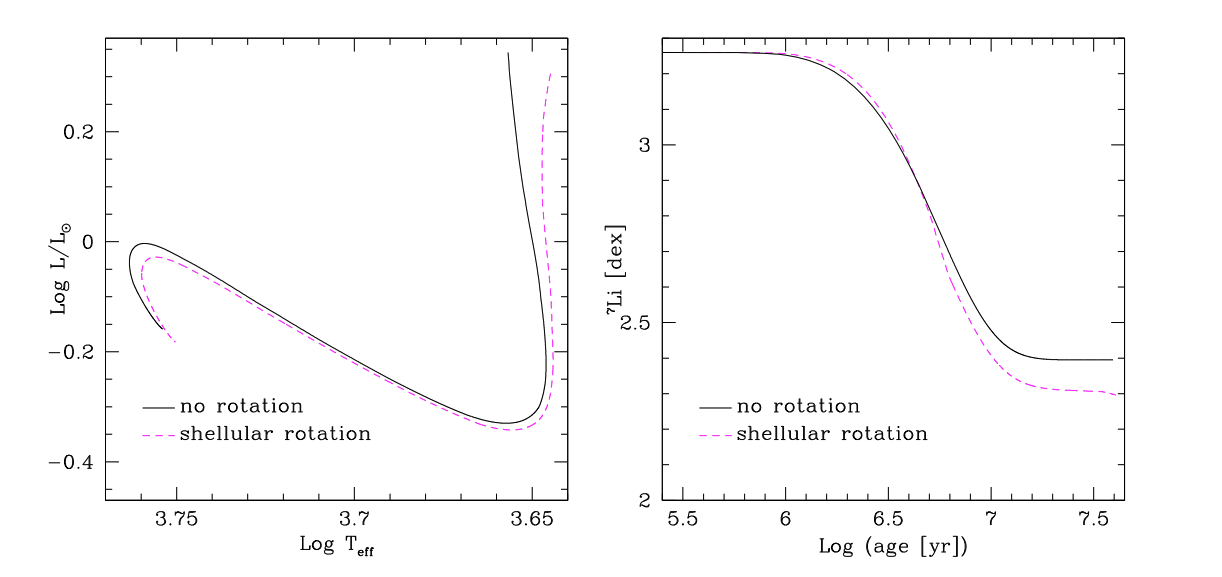
\includegraphics[width=\textwidth]{Figures/intro_figures/PMS_effect.png}
    \caption{Left: PMS HR diagram tracks of 1 M$_{\odot}$ solar metallicity models with and without rotation. The continuous line corresponds to a non-rotating model, while the dashed line corresponds to a rotating model with $\Omega = 20 \Omega_{\odot}$. The tracks end when the ZAMS is reached. Right: Surface lithium abundance with time during the PMS for the same models. Sourced from Figure 1 in \citet{eggenberger_rotation_2013}}
    \label{fig:pms_effect}
\end{figure}

Figure \ref{fig:pms_effect} (left) compares the evolutionary track of a rotating solar-type, 1M$_{\odot}$, solar metallicity, star rotating with 20 $\Omega_{\odot}$ (twenty times the mean solar surface rotation rate) against a non-rotating model of the same mass and metallicity. 
Because of the introduction of the centrifugal force, the HR path is slightly shifted towards lower effective temperatures and luminosities than a non-rotating star.

During the pre-main sequence, both the changes to the rotation impact the observed lithium abundances, which are dependent on the treatment of angular momentum transport \citep{dumont_lithium_2021}.
Figure \ref{fig:pms_effect} (right) displays the evolution of surface lithium abundance during the PMS phase for rotating and non-rotating models. 
The zero-age-main-sequence (ZAMS) surface lithium abundance of the rotating model is lower than that of the non-rotating model, indicating that including rotational effects increases lithium depletion during the PMS. 
However, during the beginning of the lithium depletion phase, the rotating model shows a slightly higher lithium content than the non-rotating one due to the centrifugal force lowering the temperature at the base of the convective envelope.

As the star develops a radiative zone at its centre, rotational mixing becomes the dominant factor in transporting lithium to deeper and hotter regions, where it is efficiently destroyed. 
This leads to a lower surface lithium abundance for the rotating model on the ZAMS compared to the non-rotating model due to the increase in differential rotation in the stellar interior during the PMS.

The duration of the disc-locking phase, which enhances differential rotation in the radiative zone, significantly impacts the sensitivity of the lithium content in rotating models. 
Longer disc lifetimes lead to lower surface lithium abundances on the ZAMS due to increased angular velocity gradients below the convective envelope, which enhance rotational mixing \citep{eggenberger_angular_2012}. 
Moreover, as the star loses more angular momentum during the longer disc-locking phase, it reaches the ZAMS with a lower surface rotational velocity, resulting in lower lithium abundance.
Therefore, a correlation between the surface velocity and lithium abundance on the ZAMS exists: stars with lower rotation rates on the ZAMS are expected to be more depleted in lithium than fast rotators on the ZAMS.

\subsubsection{Main sequence}

\begin{figure}[h]
    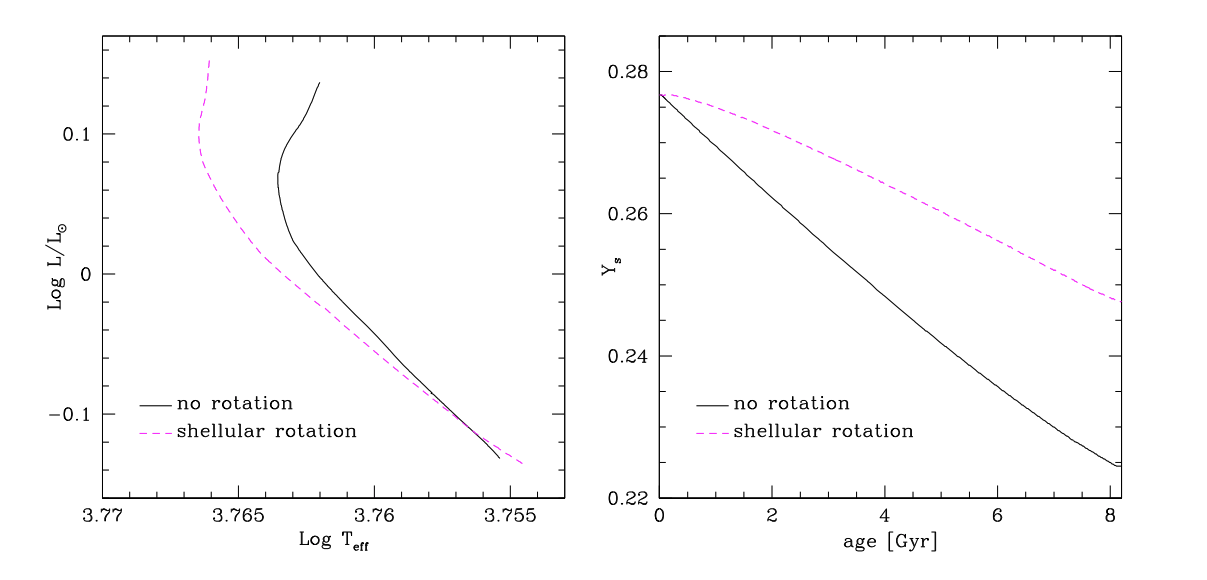
\includegraphics[width=\textwidth]{Figures/intro_figures/MS_effect.png}
    \caption{Left: MS HR diagram tracks of 1 M$_{\odot}$ solar metallicity models with and without rotation. The continuous line corresponds to a non-rotating model, while the dashed line corresponds to a rotating model with ZAMS surface velocity = 50 km/s. The tracks end when the ZAMS is reached. Right: Surface helium abundance with time during the MS for the same models. Sourced from Figure 3 in \citet{eggenberger_rotation_2013}}
    \label{fig:ms_effect}
\end{figure}

During the main sequence, rotational mixing begins to play a key role by changing the global stellar
properties. 
This is illustrated in Figure \ref{fig:ms_effect} (left), which shows the main-sequence evolution for two 1 $M_{\odot}$, solar metallicity models computed with and without rotation.
The rotating model has an initial surface velocity of 50 $km s^{-1}$

The rotating model is, like the PMS model, characterised by higher effective temperatures and slightly higher luminosities than the non-rotating model.

Figure \ref{fig:ms_effect} (right) highlights that the presence of rotational mixing counteracts the impact of atomic diffusion in the star's outer layers. 
This leads to higher helium surface abundances for the rotating model than the non-rotating model.
Consequently, the opacity in the external layers of the rotating model decreases, causing a shift towards the blue region of the HR diagram, as illustrated in Figure \ref{fig:ms_effect} (left). 
The differences in helium content between rotating and non-rotating stars become increasingly pronounced during the main sequence, resulting in significant distinctions in the HR diagram.

Furthermore, the inclusion of rotation affects the properties of the central layers of the star. As a result of rotational mixing, fresh hydrogen fuel is transported to the central core, leading to a higher central hydrogen mass fraction for rotating models than for models without rotation at a given age. This leads to an increase in the main-sequence lifetime.

\subsubsection{Post-main sequence}
Within the post-main sequence, the rotation effects are similar to the main sequence.
When rotational effects are considered, the core helium-burning phase is shifted to higher luminosity values. 
These changes are due to rotational mixing, which brings fresh hydrogen fuel into the convective core and transports helium and other H-burning products in the radiative zone.

There are no other significant enhancements in chemical abundances \citep[See Table 2. in][]{lagarde_thermohaline_2012}.
Rotation can, however, substantially affect the asteroseismic properties of low-mass red-giant stars
\citet{lagarde_thermohaline_2012, eggenberger_effects_2010}.
In particular, rotation decreases the derived stellar mass and increases the age.
Observation and identification of non-radial oscillation modes for red giants with moderate surface rotational velocities may be complicated due to non-negligible values of rotational splitting, which can be reached depending on the assumed rotation law in the convective envelope and the star's initial velocity.

\citep{eggenberger_effects_2010, lagarde_thermohaline_2012} also illustrates that the HR evolution of rotating stars can be qualitatively reproduced with enhancements to the core-overshooting parameter. 
This highlights that rotation increases the size of the convective core and changes the chemical composition of the radiative zone.



% \subsection{Photometric varability - Stellar Spots}
% \label{sec:stellar_spot_brightness_modulations}

% \subsubsection{Periodogram}
% \subsubsection{ACF}

% \subsection{Spectroscopic rotational broadenings}

% \subsection{Asteroseismology}
% \label{sec:asteroseismology}

% \subsection{Duvall Law Derivation}

% Solar/stellar oscillations represent a discrete set of observations that are sensitive to its structure and rotation. This allows us to invert the structure of a star. With a solar model, differences between its mode frequencies and observation modes are weighted averages of the differences between the Sun's structure and that of the reference model; The frequency differences can then be used to infer those structural differences. Early inversions of the Sun's structure and rotation were made using inversions described by Duvall's law \citep{duvall_jr_frequencies_1988}.\\

% Duvall's law is supplemented by analyses that linearise the full set of oscillation equations describing the stellar oscillations about a theoretical reference mode.
% The $n,\ell,m$ rotational splitting is given by:
%    \begin{equation}
%     \delta_{n,\ell,m} (\Omega) = m \beta_{n,\ell} \int^R_0 K_{n,\ell}(r) \Omega(r) \,\text{d}r
%     \label{eqn:splitting}
% \end{equation}
% where, $\delta_{n,\ell,m}$ is the $n,\ell,m$ rotational splitting of the star, $K_{n,\ell}$ is the rotational kernel of the $n,\ell$ mode (determined by the stellar model), $m$ describes the spherical harmonic order, $\Omega(r)$ is the 1D rotation profile along the radial axis and $\beta_{n,\ell}$ is a normalisation constant and $R$ is the outermost radius of the star. A more thorough interpretation of the effects of rotation \citep[See][]{aerts_asteroseismology_2010} ignores the asymptotic effects and follows the perturbation in both the horizontal and radial directions. They find a general form that is dependent on the latitudinal differential rotation.
% In practice asteroseismic constraints to latitudinal differential rotation are limited to the Sun and some solar analogues \citep{bazot}. For the sake of brevity we will focus on only radial differential rotation in the derivation of rotational splittings.

   
% As a result of space-based observations from missions like \corot{} and \kepler{} , it is now possible to measure mode splittings of stars other than the Sun. However Duvall's analysis does not hold for mixed-mode oscillations and thus the generalised form is required to probe the core properties. Here we present a derivation of the asymptotic Duvall relation.

% Can derive the asymptotic expression for the rotational splitting of p-mode frequencies very simply. Following the plane wave treatment.
% Assume hydrostatic equilibrium and consider the equation of motion.
% \todo{define div}
% \begin{equation}
%     \rho \frac{\partial \vec{v}}{\partial t} + \rho \vec{v} \ \cdot \ \nabla \vec{v} = \nabla p +\rho \vec{g}
%     \label{eqn:eom}
% \end{equation}
% For now we will ignore the full equations of stellar hydrostatic equilibrium.\\
% Now consider an Eulerian perturbation about the equilibrium state
% \begin{equation}
%     p(\vec{r},t) = p_0(\vec{r}) + p' (\vec{r},t)
% \end{equation}
% It can be convenient to use the Langrangian perturbation. In the reference frame following the motion: if an element of gas is moved from $\vec{r_0}$ to $\vec{r_0}$ + $\delta\vec{r}$ the change is pressure is given as:\\
% \begin{equation}
%     \delta p (\vec{r}) = p(\vec{r_0} + \delta \vec{r}) - p_0(\vec{r_0}) + \delta r \cdot \nabla p_0 - p_0(r_0)
%      = p'(r_0) + \delta \vec{r} \cdot \nabla p_0 
% \end{equation}
% Note that the velocity is given by the time derivative of the displacement $\vec{\delta r}$,
% \begin{equation}
%     \vec{v} = \frac{\partial \vec{\delta r}}{\partial t}
% \end{equation}
% Equations for the perturbation are obtained by inserting these expressions into the full equations and neglect quantities of higher-order terms. The equation of motion becomes
% \begin{equation}
%     \rho_0 \frac{\partial^2 \delta\vec{r}}{\partial t^2} = \rho_0 \frac{\partial \vec{v}}{\partial t} = - \nabla p' + \rho_0 \vec{g}' + \rho ' \vec{g_0}
% \end{equation}
% Where, $\vec{g}' = -\nabla \Phi' (\Phi')$ satisfies the perturbed Possion's equation. And the continuity equation becomes 
% \begin{equation}
%     \frac{\partial \rho '}{\partial t} + \dive (\rho_0 \vec{v}) = 0
%     \label{eom_int}
% \end{equation}
% or by integrating with respect to time
% \begin{equation}
%     \rho' + \dive (\roh \vec{\delta r}) = 0
%     \label{eqn:ce}
% \end{equation}
% \subsubsection{Acoustic Waves}
% As the simplest equilibrium situation, consider the spatially homogeneous case. All derivatives of equilibrium quantities vanish. Here all derivatives of equilibrium quantities vanish. According to the equation of motion: gravity must be negligible. Such a situation clearly cannot be realized exactly. Consider the case where the equilibrium structure varies slowly compared with the oscillations and this becomes a reasonable approximation. Also neglect the perturbation to the gravitational potential and assume adiabatic approximation:
% \begin{equation}
%     \delta p = \frac{\Gamma_{1,0} p_0}{\rho_0} \delta \rho
% \end{equation}
% Equation \ref{eqn:eom} gives:
% \begin{equation}
%     \rho_0 \frac{\partial^2 \delta\vec{r}}{\partial t^2} = -\nabla p'
% \end{equation}
% Or by taking the divergence:
% \begin{equation}
%     \rho_0 \frac{\partial ^2}{\partial t^2} (\dive \ \vec{\delta r}) = - \nabla^2 p'
%     \label{eqn:3.43}
% \end{equation}
% div \vec{$\delta$ r} can be eliminated using the continuity equation \ref{eqn:ce}, and $p$' can be expressed in terms of $\rho$' using the adiabatic relation:
% \begin{equation}
%     \frac{\partial^2 \rho}{\partial t^2} = \frac{\Gamma_{1,0} p_0}{\rho_0} \nabla^2 \rho' = c_0^2 \nable^2 \rho'
%     \label{eqn:relation}
% \end{equation}
% Where
% \begin{equation}
%     c_0^2 = \frac{\Gamma_{1,0} p_0}{\rho_0}
% \end{equation}
% Is the sound speed. This equation has the form of the wave equation and has solutions in the form of plane waves:
% \begin{equation}
%     \rho' = a \exp [i (\vec{k} \cdot \vec{r} - \omega t)]
% \end{equation}
% By substituting this into \ref{eqn:relation} we obtain:
% \begin{equation}
%     -\omega^2 \rho' = c_0^2 \dive (i \vec{k} \rho ') = -c_0^2 \vert \vec{k} \vert ^2 \rho'
% \end{equation}
% This is a solution provided $\omega$ satisfies the dispersion relation
% \begin{equation}
%     \omega^2 = c_0^2 \vert \vec{k} \vert ^2
%     \label{eqn:nondisp}
% \end{equation}

% \subsubsection{The effect of rotation}

% We need to reconsider the derivation of the perturbation equations and include the effects of a velocity field. Assume that the equillibrium structure is stationary so all time derivatives vanish. Even with this assumption the determination of the equilibrium structure is non-trivial, owing to distortion caused by the velocity fields (e.g.
% due to centrifugal effects in a rotating star). However if we assume that the velocity $\vec{v_0}$ in the equilibrium state is sufficiently slow that terms quadratic in $\vec{v_0}$ can be neglected. The continuity equation \ref{eqn:ce} gives, because of the assumed stationarity:
% \begin{equation}
%     \dive (\rho_0 \vec{v_0}) = 0
%     \label{eqn:assum}
% \end{equation}

% Also the equation of motion (\ref{eqn:eom}) reduces to:
% \begin{equation}
%     0= -\nabla p_0 + \rho_0 \vec{g}_0
% \end{equation}
% Equation of hydrostatic support is unchanged.
% The velocity at a given point in space can be written:
% \begin{equation}
%     \vec{v} = \vec{v_0} + \vec{v}'
% \end{equation}
% Where $\vec{v}$ is the Eulerian velocity perturbation. The displacement $\vec{\delta r}$ is determined relative to the moving equillibrium fluid; related to the velocity perturbation by:
% \begin{equation}
%     \frac{\der \vec{\delta r}}{\der t} = \vec{\delta v} = \vec{v}' + (\delta r \cdot \nabla) \vec{v_0}
%     \label{eqn:8.6}
% \end{equation}
% Where $\vec{v}$ is the Lagrangian velocity perturbation and d/dt is the material time derivative. Furthermore:
% \begin{equation}
%     \frac{\der \vec{\delta r}}{\der t} = \frac{\partial \vec{\delta r}}{\partial t} + (\vec{v} \cdot \nabla) \delta r
%     \label{eqn:8.7}
% \end{equation}
% Using both of these equations the perturbed continuity equation can be written
% \begin{equation}
%     0 = \frac{\partial \rho ' }{\partial t} + \dive (\rho' \vec{v_0} + \rho_0 \vec{v'})
% \end{equation}
% \begin{equation}
%     0 = \frac{\partial}{\partial t} [\rho' + \dive (\rho_0 \delta r)] + \dive [\rho' \vec{v_0} + \rho_0 [ (\vec{v_0} \cdot \nabla)\vec{\delta r} - (\delta r \cdot \nabla)\vec{v_0}]]
% \end{equation}
% After some massaging, using \ref{eqn:assum} this can be reduced to:
% \begin{equation}
%     \frac{\partial A}{\partial t} + \dive (A \vec{v_0}) = 0
% \end{equation}
% Where
% \begin{equation}
%     A = \rho' + \dive (\rho_0 \vec{\delta r})
% \end{equation}
% This may also be written using Equation \ref{eqn:assum}
% \begin{equation}
%     \rho_0 \frac{\der}{\der t} \left(\frac{A}{\rho_0}\right) =0
% \end{equation}
% From which we can conclude that A = 0 and as such Equation \ref{eom_int} holds. This may now be written from Equation \ref{eqn:8.6}:
% \begin{equation}
%     \rho_0 \frac{\der \vec{\delta r}}{\der t} = - \nabla p' + \rho \vec{g}' + \rho' \vec{g_0}
% \end{equation}
% Or using Equation \ref{eqn:8.7}:
% \begin{equation}
%     \rho_0 \frac{\partial ^2 \vec{\delta r}}{\partial t^2} + 2 \rho_0 (\vec{v_0} \cdot \nabla) \left( \frac{\partial \vec{\delta r}}{\partial t}\right) = - \nabla p' + \rho_0 \vec{g}' + \rho' \vec{g_0}
% \end{equation}
% which replaces Equation \ref{eqn:3.43}. As the equilibrium structure is independent of time we may still separate the time dependence as an oscillatory term ($\exp (-i \omega t)$). Using solutions of this form the equations of motion become:
% \begin{equation}
%     - \omega^2 \rho_0 \vec{\delta r} - 2 i \omega \rho_0 (\vec{v_0} \cdot \nabla) \vec{\delta r} = -\nabla p' + \rho_0 \vec{g'} + \rho' \vec{g_0}
% \end{equation}
% Where the first term on the LHS corresponds to the Coriolis force and is neglected in this work. Using the acoustic wave approximations as before we obtain the dispersion relation for a plane sound wave as:
% \begin{equation}
%     \omega^2  c^2 \vert \vec{k} \vert^2 + 2 m \omega \Omega
%     \label{eqn:disp}
% \end{equation}
% This is treated as a perturbation to the Duvall relation.
% \subsubsection{The Duvall relation}
% One of the most important results of asymptotic analysis is the Duvall relation \citep{duvall_jr_frequencies_1988} from analysis of observed frequencies of solar oscillation. Starting with the dispersion relation for a plane sound wave, neglecting self-gravity, in a slowly rotating star. First consider the non-rotating case. Take Equation \ref{eqn:nondisp} as our dispersion relation and writing $\vert \vec{k}\vert^2 = k_r^2 + k_h^2$. Where $k_h$ is the length of the horizontal component of the wave vector and $k_r$ is the radial component. For a wave corresponding to a mode oscillation, $k_h$ is given by:
% \begin{equation}
%     \frac{\ell (\ell +1)}{r^2} = k_h^2
% \end{equation}
% Dropping subscripts on equilibrium quantities $k_r^2$ can be written 
% \begin{equation}
%     k_r^2 = \frac{\omega^2}{c^2} - \frac{L^2}{r^2}
% \end{equation}
% Where $L^2 = \ell (\ell + 1)$. The condition for a standing wave is roughly that:
% \begin{equation}
%     \int ^R _{r_{t}} k_r \der r = n \pi
%     \label{eqn:standing}
% \end{equation}
% Where $r_{t}$ is the inner turning point of the oscillation mode. A more careful analysis shows that $n$ should be replaced with $n+\alpha$ where $\alpha$ takes care of the behaviour near the lower turning point $r_{t}$ and at the surface. We can combine these into the Duvall relation:
% \begin{equation}
%     \int ^R _{r_{t}} \left( 1 - \frac{L^2}{\omega^2} \frac{c^2}{r^2} \right)^{1/2} \frac{\der r}{c} = \frac{(n + \alpha \pi)}{\omega}
% \end{equation}
% \subsubsection{Effect of a perturbation on acoustic-mode frequencies}
% Variations on the Duvall law from small perturbation reflect more general expressions. These perturbations can come in the form of changes to gravitational potential, changes in model/sound speed and rotation. Starting with the dispersion relation for a plane sound wave, with the addition of some \textbf{radial} perturbation $\delta_r a(r)$:
% \begin{equation}
%     \omega^2 = c^2 \vert \vec{k}\vert^2 + \delta_r a(r)
% \end{equation}
% Following the same analysis as above $k_r^2$ can be written as:
% \begin{equation}
%     k_r = \left(\frac{\omega^2}{c^2} - \frac{L^2}{r^2} - \frac{1}{c^2} \delta_r a\right)^{1/2}
% \end{equation}
% Expanding this and taking first order terms
% \begin{equation}
%     k_r \simeq \frac{\omega}{c} \left[ \left(1-\frac{L^2 c^2}{\omega^2 r^2}\right)^{1/2} - \frac{1}{2\omega^2} \left(1 - \frac{L^2 c^2}{\omega^2 r^2}\right)^{-1/2} \delta_r a \right]
% \end{equation}
% Substituting this into Equation \ref{eqn:standing}, using the $\alpha$ term to correct for boundary effects, we obtain \begin{equation}
% \frac{(n+\alpha) \pi}{\omega} \simeq \int^R _{r_t}   \left( 1 - \frac{L^2 c^2}{\omega^2 r^2}\right)^{1/2} \frac{\der r}{c} - \frac{1}{2 \omega^2} \int^R _{r_t}  \left(1 - \frac{L^2 c^2}{\omega^2 r^2}\right)^{-1/2} \delta_r a \frac{\der r}{c}
% \end{equation}
% If we neglect the term in $\delta_r a $ we retain the Duvall law. This reflects a perturbation on the Duvall law.
% We can now find the effect on the oscillation frequencies of the perturbation. Assume that the result is to change the frequency from $\omega$ to $\omega + \delta \omega$. $\alpha$ here is generally a function of $\omega$ by multiplying the perturbed Duvall law by $\omega$ and  perturbing is we obtain:
% \begin{align}
% \pi \frac{\der \alpha}{\der \omega} \delta \omega &= \delta \omega \int^R _{r_t}  \left( 1 - \frac{L^2 c^2}{\omega^2 r^2}\right)^{1/2} \frac{\der r}{c} + \omega \int^R _{r_t}  \left( 1- \frac{L^2 c^2}{\omga^2 r^2}\right)^{-1/2} \frac{L^2 c^2}{\omega^2 r^2} \frac{\delta \omega}{\omega}\frac{\der r}{c}\\
% &-\frac{1}{2 \omega} \int^R_{r_t}  \left( 1 - \frac{L^2 c^2}{\omega^2 r^2} \right)^{-1/2} \delta_r a \frac{\der r}{c}
% \label{eqn:modifiedduvall}
% \end{align}
% From this we obtain the generalised expression:
% \begin{equation}
%     S \frac{\delta \omega}{\omega} \simeq \frac{1}{2 \omega^2} \int^R _{r_t}  \left(1 - \frac{L^2 c^2}{\omega^2 r^2}\right)^{-1/2} \delta_r a \frac{\der r}{c}
% \end{equation}
% where
% \begin{equation}
%     S = \int^R _{r_t}  \left( 1 - \frac{L^2 c^2}{\omega^2 r^2}\right)^{-1/2} \frac{\der r}{c} - \pi \frac{\der \alpha}{\der \omega}
% \end{equation}

% \subsubsection{Effect of rotation on the Duvall relation}
% Assume a radial rotation profile and that is is small the modified rotation Duvall relation can be written:
% \begin{equation}
%     \pi \frac{n+\alpha}{\omega} = \int^R_{r_t} \left(1 - \frac{L^2 c^2}{\omega^2 r^2}\right)^{1/2} \frac{\der r}{c} - \frac{m}{\omega} \int^R_{r_t}  \left(1 - \frac{L^2 c^2}{\omega^2 r^2}\right)^{-1/2} \Omega(r) \frac{\der r}{c}
% \end{equation}
% Furthermore the rotational splitting can be described by the following
% \begin{equation}
%     S \delta \omega \simeq m \int^R _{r_t} \left(1 - \frac{L^2 c^2}{\omega^2 r^2}\right)^{-1/2} \Omega(r) \frac{\der r}{c}
%     \label{eqn:final}
% \end{equation}
% \subsubsection{Inverting the Duvall relation}
% Given Equation \ref{eqn:final} it is straight forward to consider $(1 - L^2c^2/r^2\omega^2)$ as a Kernel like (weighting) term. Inverting the stellar rotation profile from here requires either forward modelling or an inversion technique such as optimised local averages, regularised least square or forward modelling to obtain the rotation profile.\\
% For higher-order p modes Equation \ref{eqn:final} can be further simplified and $(1 - L^2c^2/r^2\omega^2)$ can be crudely approximated by 1. The rotational splitting relation be written:
% \begin{equation}
%     \delta_{n,\ell,m} \simeq m \frac{\int^R _{r_t}\Omega (r)\frac{\der r}{c}}{\int^R _{r_t}\frac{\der r}{c}}
% \end{equation}
% This is dependent on the model/structure of the star but is straight forward to forward model and obtain the stellar structure. The inversion is dependent on the observed modes and thus the evolutionary state of the star.


% \subsection{Average core and surface rotation rates}

%  Inverting a stellar rotation profile given measured rotational splittings is an ill-posed problem. 
%  State-of-the-art methods involve the use of linear inversion techniques. Examples of these methods include regularised least squares \citep[RLS;][]{christensen-dalsgaard_comparison_1990}, which has proven successful for the case of the Sun, and Optimally Localised Averages \citep[OLA;][]{pijpers_faster_1992,pijpers_sola_1994},
% which has also been used to accurately infer the core and surface rotation rates of stars other than the Sun. 
% Both methods rely on having a good best-fitting model to describe the sensitivity of modes to rotation at different radii. The sensitivity of rotational splittings to differing parts of a star is shown by the rotation kernels. Observational uncertainties enter any given inversion technique both from the asteroseismic rotational splittings and constraints on the stellar model. The oscillation frequencies and spectroscopic constraints underpin these uncertainties; the uncertainty in the constraints is due to the precision of the stellar model and thus the rotational kernels.\\

% OLA inversions are limited by the fact that they rely on extremely low resolution rotation profiles. Often only two measured points are available. This is a necessary condition as OLA becomes numerically unstable with increased resolution, yet is insufficient to describe the rotational gradient throughout a star.
% RLS inversions differ in that they are able to provide a mean rotational profile of a star owing to the rotational splitting. 
% However, between the well-constrained core and surface rotation rates, the mean rotational profile is limited by the regularising smoothing constant. 
% RLS can only inform the mean rotational profile according to this smoothing parameter and the inferred core and surface rotational rates are dependent on this regularisation.
%  Further constraints on the method of increased angular momentum transport post main-sequence could be implied through higher resolution inversions of the rotational profile.


% \subsection{OLA}
% \subsubsection{MOLA}
% \subsubsection{SOLA}


%todo DISCUSS WHY ONLY LOW MASS, BELOW 6500K YOU AVOID PULSATORS ETC WHICH MAKE MEASURING ROTATION PERIOD VERY HARD TO DO.
\section{Todo}
Write section on ways that observations of rotation are made - precise techniques.
\begin{itemize}
    \item Rotation period from light curves - acf method and periodgram
    \item Doppler broadening spectroscopy
    \item Asteroseismic inference of rotation rate - OLA techniques + Forward modelling
\end{itemize}

% \bibliography{references}

